\documentclass[aspectratio=169, 9pt, handout]{beamer}

%\transdissolve[duration=0.2] % Only works with Adobe Acrobat

% Some important packages
\usepackage{epstopdf}
\usepackage{ulem} % sout
\hypersetup{colorlinks=false, allcolors=purple}
\usepackage{booktabs}
\linespread{1.3}
\usepackage{tabularx,multirow}
\usepackage{makecell} % For makecell within tables
\usepackage{geometry}
\usepackage{fancybox}
\usepackage{algorithm2e}
\usepackage{amsmath, amssymb}
% Mathematical functions
% DELETED!
\renewcommand{\Pr}[1]{{\mathbb{P}\left(#1\right) }}
% DELETED!
% DELETED!
% DELETED!
% DELETED!
% DELETED!

% DELETED!
\newcommand{\sufstats}[1]{s\left(#1\right)}
\renewcommand{\exp}[1]{\mbox{exp}\left\{#1\right\}}
\renewcommand{\log}[1]{\mbox{log}\left\{#1\right\}}
\newcommand{\transpose}[1]{{#1}^\mathbf{t}}
\renewcommand{\t}[1]{\transpose{#1}}

\newcommand{\s}[1]{\sufstats{#1}}
\newcommand{\SUFF}{\mathcal{S}}
\newcommand{\Suff}{\mathbf{S}}
\newcommand{\suff}{\mathbf{s}}

\renewcommand{\beta}{\theta}
\newcommand{\weight}{\mathbf{w}}
\newcommand{\Weight}{\mathbf{W}}

% Objects
% DELETED!
% DELETED!
\newcommand{\Graph}{\mathbf{G}}
\newcommand{\graph}{\mathbf{g}}
\newcommand{\GRAPH}{\mathcal{G}}
\newcommand{\Adjmat}{Y}
\newcommand{\adjmat}{y}
\newcommand{\ADJMAT}{\mathcal{Y}}

\newcommand{\INDEPVAR}{\mathcal{X}}
\newcommand{\Indepvar}{X}
\newcommand{\indepvar}{x}

\newcommand{\normconst}{\kappa\left(\params, \Indepvar\right)}

\graphicspath{{./figures/}{.}{./terms/}}


%% NEED THIS FOR CANCY TEX
\usepackage{pstricks}

% Colors
\definecolor{USCCardinal}{HTML}{990000} % 153 0 0 in RGB
\definecolor{USCGold}{HTML}{FFCC00}
\definecolor{USCGray}{HTML}{CCCCCC}

% \bibliography{bibliography.bib}

\def\ergmito{ERGM\textit{ito}}
\def\ergmitos{\ergmito{}\textit{s}}
% Mathematical functions
\newcommand{\isone}[1]{{\boldsymbol{1}\left( #1 \right)}}
\renewcommand{\Pr}[1]{{\mathbb{P}\left(#1\right) }}
\newcommand{\f}[1]{{f\left(#1\right) }}
\newcommand{\Prcond}[2]{{\mathbb{P}\left(#1\vphantom{#2}\;\right|\left.\vphantom{#1}#2\right)}}
\newcommand{\fcond}[2]{{f\left(#1|#2\right) }}
\newcommand{\Expected}[1]{{\mathbb{E}\left\{#1\right\}}}
\newcommand{\ExpectedCond}[2]{{\mathbb{E}\left\{#1\vphantom{#2}\right|\left.\vphantom{#1}#2\right\}}}
\renewcommand{\exp}[1]{\mbox{exp}\left\{#1\right\}}

\newcommand{\Likelihood}[2]{\text{L}\left(#1 \left|\vphantom{#1}#2\right.\right)}

\newcommand{\loglik}[1]{l\left(#1\right)}


% Mathematical Annotation -------------------------------
% Modify this so that it matches the P01 convention overall

% Tree
\newcommand{\phylo}{\Lambda{}} % The actual tree
\newcommand{\aphylo}{D{}}      % The annotated phylogenetic tree
\newcommand{\aphyloObs}{\tilde \aphylo{}} % The observed annotated phylogenetic tree
\newcommand{\parent}[1]{\mathbf{p}\left(#1\right)}
\newcommand{\offspring}[1]{\mathbf{O}\left(#1\right)}
\newcommand{\nodes}{\mathcal{N}{}}
\newcommand{\edges}{\mathcal{E}{}}

\newcommand{\class}[1]{C_{#1}{}}

% Annotations
\newcommand{\Ann}{\mathbf{X}{}} % Matrix of "real" annotations
\newcommand{\ann}[1]{x_{#1}{}} % single element of "real" annotations
\newcommand{\constraints}{\mathcal{C}{}} % Taxon constraints

% Obs Annotations
\newcommand{\AnnObs}{\mathbf{Z}{}}%{Z{}} \mathbf{X}^{obs}{}
\newcommand{\annObs}[1]{z_{#1}{}}%{z{}}  x_{#1}^{obs

% Pred. Annotations
\newcommand{\AnnPred}{\hat X{}}
\newcommand{\annPred}[1]{\hat x_{#1}}

% Leaf nodes
\newcommand{\Leaf}{L{}}

% Shortest path
\newcommand{\Geodesic}{\text{T}{}}
\newcommand{\geodesic}{\tau{}}

\newcommand{\Params}{\Omega{}}
\newcommand{\params}{\omega{}}

% Parameters
\newcommand{\gain}{\mu_{01}{}}
\newcommand{\loss}{\mu_{10}{}}
\newcommand{\misszero}{\psi_{01}{}}
\newcommand{\missone}{\psi_{10}{}}
\newcommand{\proot}{\pi}


% New notation ------------------------------------------------------------------
\newcommand{\expo}{E}
\newcommand{\Expo}{\mathbf{\expo{}}}
\newcommand{\expod}[1]{\expo_{#1}^D}
\newcommand{\expoc}[1]{\expo_{#1}^C}
\newcommand{\expoi}[1]{\expo_{#1}^I}

\newcommand{\covar}{\mathbf{x}}
\newcommand{\Covar}{\mathbf{X}}
\newcommand{\latent}{\mathbf{z}}
\newcommand{\Latent}{\mathbf{z}}

\newcommand{\Event}{\mbox{P}}
\newcommand{\pset}[1]{\mathcal{P}\left(#1\right)}
\newcommand{\size}[1]{\left|#1\right|}

\newcommand{\logit}[1]{\mbox{logit}^{-1}\left(#1\right)}
% -------------------------------------------------------------------------------

% Neat trick to change the mode mid-presentation
% https://tex.stackexchange.com/questions/91691/beamer-set-mode-mid-presentation?rq=1
\makeatletter
\newcommand\changemode[1]{%
	\gdef\beamer@currentmode{#1}}
\makeatother


% Styles
\usepackage{xcolor}
\usepackage{colortbl}
\definecolor{suffstat}{RGB}{10,159,0}
\definecolor{normconst}{RGB}{87,38,231}
\setbeamercolor{conclusions}{bg=usclightgray!60!white, fg=uscdarkgray}

% Noice!
\usetheme{usckeck}

\title[SNA Meets Phylogenetics]{%
	Triads, Dyads, and Gene Functions\\When Social Network Analysis Meets Phylogenetics
}
\author[GGVY -- \href{vegayon@usc.edu}{vegayon@usc.edu}]{George G Vega Yon, Ph.D.}
\institute[USC-PREVMED]{University of Southern California, Department of Preventive Medicine}
\date{NY Genome Center\\December 10, 2020}

% Some definitions
\def\cursection{\frame{\frametitle{Contents}\tableofcontents[current]}}
\newcommand{\ergmpkg}[0]{\texttt{ergm}}
\newcommand{\ergmitopkg}[0]{\texttt{ergmito}}
\newcommand{\aphylopkg}[0]{\texttt{aphylo}}
\graphicspath{{.}{fig/}{fig-whoami/}{fig-struct-test/}}

\usepackage{media9}


% ------------------------------------------------------------------------------
% ------------------------------------------------------------------------------
% --------------------------- END OF PREAMBLE ----------------------------------
% ------------------------------------------------------------------------------
% ------------------------------------------------------------------------------
\setbeamertemplate{note page}[plain]
%\setbeameroption{show notes}
\usepackage{pgfpages}
% \setbeameroption{show notes on second screen}

\newcommand{\hlc}[2]{{\only<#1>{\cellcolor{gray!50}#2}}}
\newcommand{\nhlc}[2]{{\only<#1>{#2}}}
\newcommand{\hlcAlt}[2]{\alt<#1>{\cellcolor{gray!50}#2}{#2}}

\newcommand{\byside}[3]{\begin{minipage}[t]{#1\linewidth}%
		\bigskip
		\centering%
		\shadowbox{\Large #2}\hfill\\\bigskip%
		#3%
\end{minipage}}

\begin{document}

% ------------------------------------------------------------------------------
\begin{frame}%[noframenumbering]
\maketitle
\vspace{-.5cm}
%\begin{center}
%	\begin{minipage}[m]{.5\linewidth}
%		\color{uscgold}\centering
%		\textbf{Committee} \\
%		Paul~Marjoram (chair), Kayla~de~la~Haye, Paul~D~Thomas, Duncan~C~Thomas, Emilio~Ferrara
%	\end{minipage}
%
%\end{center}
\end{frame}

%% ------------------------------------------------------------------------------
%\begin{frame}
%\frametitle{What motivates my research}
%
%\centering
%
%\begin{center}
%\large
%\textcolor{usccardinal}{
%Essays on Bioinformatics and Social Network Analysis
%\linebreak{\small Statistical and Computational Methods for Complex Systems}
%}
%\end{center}\pause
%
%\begin{itemize}
%\item We live in a non-{\it IID} world.\pause
%\item Sometimes, we cannot understand a process unless we look at it as a whole.\pause
%\item But, while ``the whole'' may be difficult to analyze...\\
%\hfill \pause{\it modern} statistical and computational tools cap help us cope with that.
%\end{itemize}
%\end{frame}

\begin{frame}[c]
	%	\frametitle{George G. Vega Yon}
	
	\Large My work sits at the intersection between...\normalsize
	
	
	\uncover<2->{\byside{.32}{Statistics}{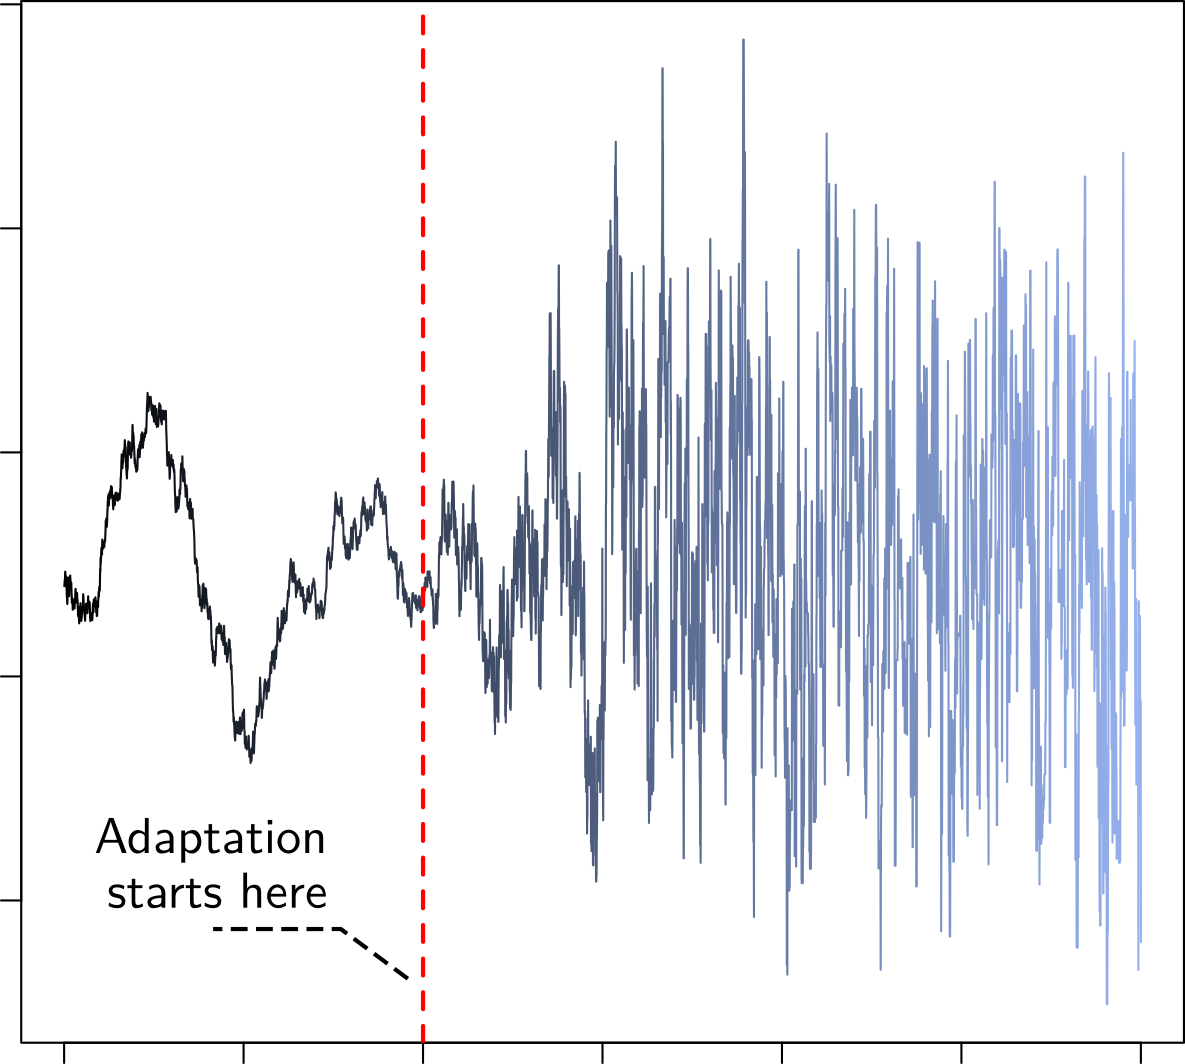
\includegraphics[width=.8\linewidth]{mcmc.png}\\Bayesian, Non-parametric, Spatial}}
	\uncover<3->{\byside{.32}{Computer Science}{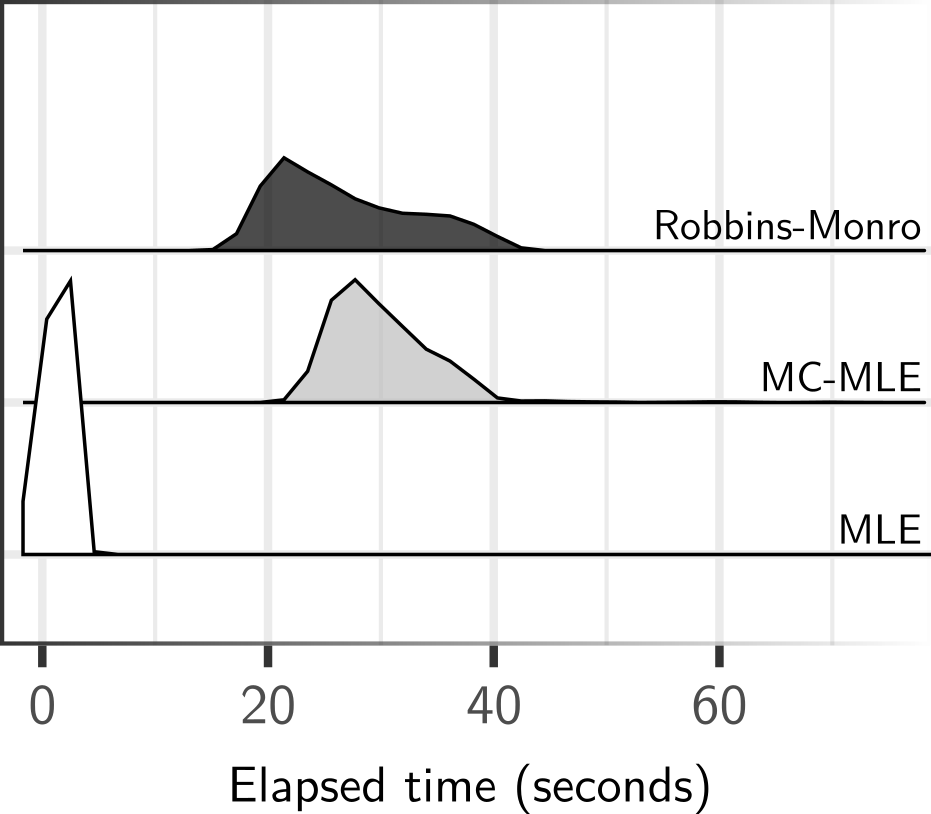
\includegraphics[width=.8\linewidth]{time.png}\\ parallel computing, HPC, software}}
	\uncover<4->{\byside{.32}{Complex Systems}{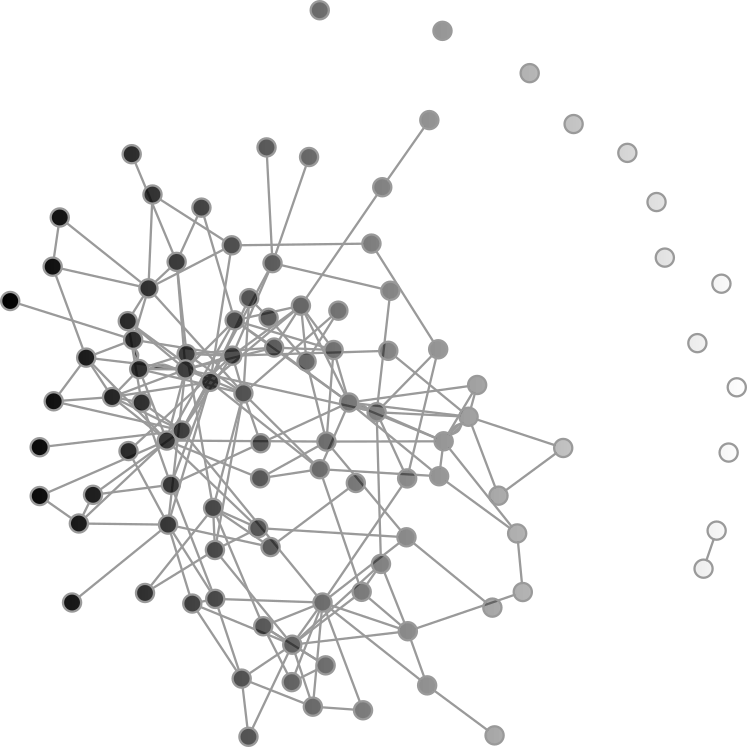
\includegraphics[width=.8\linewidth]{complex.png}\\social, biological, technical}}
	
	
\end{frame}

\frame{\frametitle{Contents}
	\tableofcontents
	\vfill
	You can download the slides from\large{} {\color{usccardinal}\href{https://ggv.cl/slides/uai-fic}{ggv.cl/slides/uai-fic}}\normalsize
}

%\begin{frame}
%		\Large Career path\bigskip\normalsize
%	\begin{center}
%		\begin{tabular}{*{3}{m{.25\linewidth}<\centering}}
%			Master Economics and Public Policy & %
%			Master in Social Science \linebreak  Economics &
%			PhD in Biostatistics \linebreak Statistical Computing 
%			\\
%			(UAI)  & (Caltech) & (USC)
%		\end{tabular}
%	\end{center}\bigskip
%\end{frame}



% ------------------------------------------------------------------------------
\section{Parsimonious modeling of gene functional evolution}

\begin{frame}[t]
\usebeamertemplate{section intro}{}{}
\textcolor{uscgold}{
\Large {\bf Parsimonious modeling of gene functional evolution} \vskip0.25em
\large \textit{Joint with}: Paul D Thomas, Paul Marjoram, Huaiyu Mi, Duncan Thomas, and John Morrison \\
(\small Published at \textit{PLOS Computational Biology})
}
\end{frame}


% ------------------------------------------------------------------------------

\begin{frame}[c]
%	\frametitle{Uncovering the role of genes}
	
	\Large Is gene \textit{XYZ} involved in process \textit{ABC}?\normalsize\bigskip
	
	\begin{minipage}[t]{.33\linewidth}
		\centering
		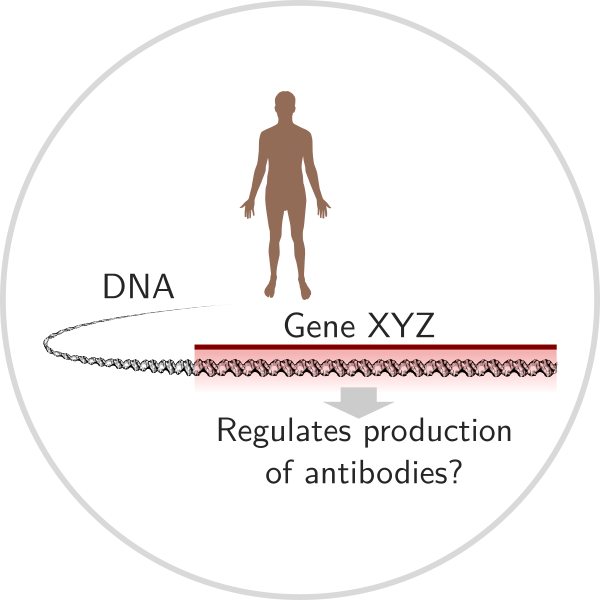
\includegraphics[width=1\linewidth]{aphylo-data-0.png} \\
		Complex to directly assess
	\end{minipage}\hfill
	\uncover<2->{\begin{minipage}[t]{.33\linewidth}
		\centering
		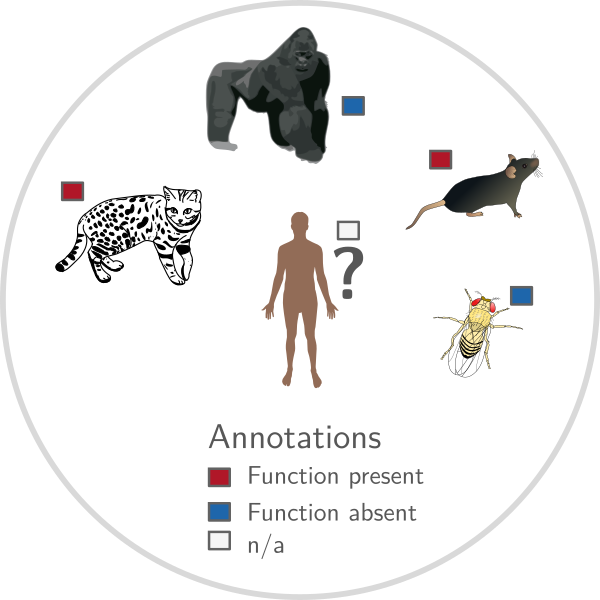
\includegraphics[width=1\linewidth]{aphylo-data-1.png}\\
		But we may know from other species
	\end{minipage}}\hfill
	\uncover<3->{\begin{minipage}[t]{.33\linewidth}
		\centering
		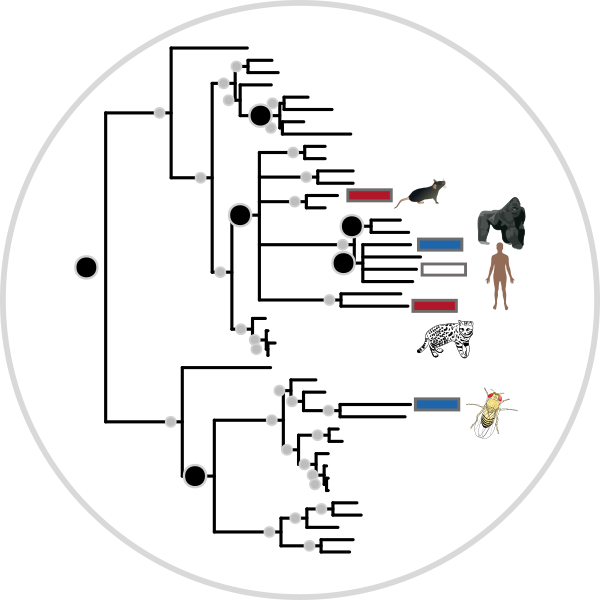
\includegraphics[width=1\linewidth]{aphylo-data-2.png}\\
		And we further know how these \textit{genetically} connected
	\end{minipage}}\hfill
	
\bigskip\uncover<4>{\raggedleft\Large ... let's rephrase the question. \normalsize}

\end{frame}

\begin{frame}[c,label=aphylo-prob-diagram]
	\begin{center}
		\normalsize Is the human gene \textbf{XYZ} involved in process \textbf{ABC}, \uline{given what we know about that for other \textit{related} species}?
	\end{center}
	
	\begin{figure}
		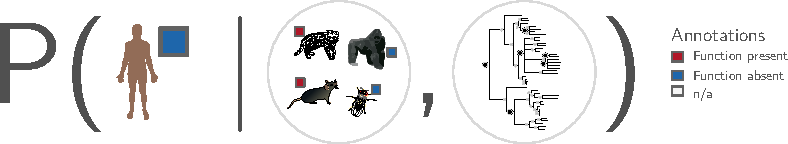
\includegraphics[width=.9\linewidth]{aphylo-data-probability.pdf}
	\end{figure}\pause
	\Large \bigskip\hfill... Where is all this data?\normalsize


\vfill\hfill\hyperlink{aphylographicalview}{\beamergotobutton{more}}

\end{frame}

\begin{frame}[c,label=geneontology]
	\frametitle{The Gene Ontology Project}
	\begin{minipage}[m]{.33\linewidth}
		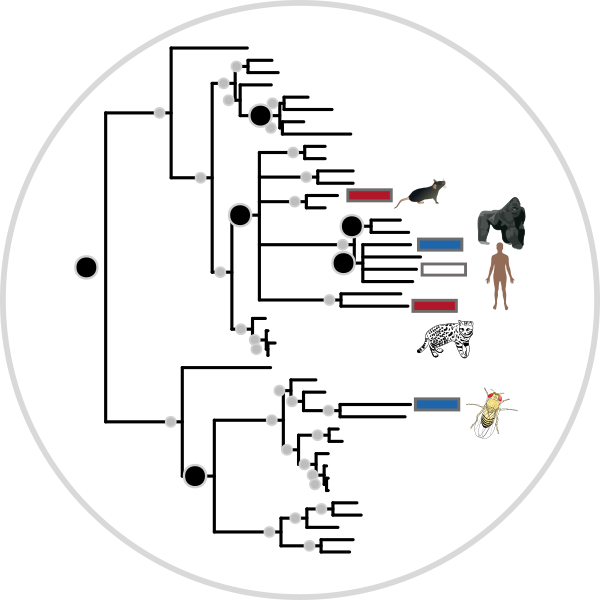
\includegraphics[width=1\linewidth]{aphylo-data-2.png}
	\end{minipage}\hfill
	\begin{minipage}[m]{.66\linewidth}
		\begin{figure}
		
\includegraphics[width=.5\linewidth]{go-logo.png}
		\end{figure}
	\begin{itemize}
		\item<2-> $\sim$ 15,000 phylogenetic trees		
		\item<3-> $\sim$ 8 million annotations
		\item<4-> $\sim$ 600 thousand on human genes
		\item<5-> $\sim$ $<$ 10\% are based on experimental evidence... \uncover<6->{Improving our knowledge on genetics is fundamental for advancing Biomedical Research}
	\end{itemize}
	\end{minipage}
\vfill \hfill
\Large \uncover<7->{Only on 2021, 2,500+ Cancer papers using the GO \href{https://scholar.google.com/scholar?as\_ylo=2021\&q=\%22gene+ontology\%22+Cancer\&hl=en\&as_sdt=0,5}{(Google Scholar)}}\normalsize\\
\hfill\hyperlink{go-functions-types}{\beamergotobutton{more}}

\end{frame}

%--------------------------------------------------------------------------------
\newcommand{\oinclude}[2]{\only<#1>{\includegraphics[width=\tmpwdth,clip,trim={0 0 0 2cm}]{#2}}}


%%-------------------------------------------------------------------------------
%\begin{frame}
%	\frametitle{An evolutionary model of gene functions}
%	
%	Imagine a relay race...
%	\begin{figure}
%		\includegraphics[width=.55\linewidth]{800px-2019-09-01_ISTAF_2019_4_x_100_m_relay_race_(Martin_Rulsch)_10.jpg}
%		\caption{ISTAF 2019 4 x 100 m relay race (Martin Rulsch, \href{https://commons.wikimedia.org/wiki/File:2019-09-01_ISTAF_2019_4_x_100_m_relay_race_(Martin_Rulsch)_10.jpg}{wikimedia})}
%	\end{figure}
%	
%\end{frame}

%--------------------------------------------------------------------------------
%\newcommand{\oinclude}[2]{\only<#1>{\includegraphics[width=\tmpwdth,clip,trim={0 0 0 2cm}]{#2}}}

\begin{frame}[t, label=aphylo-good]
	\frametitle{An evolutionary model of gene functions}
	
	\begin{minipage}[m]{.34\linewidth}
		\small
		%	The AUC for this analysis is 0.91 and the Mean Absolute Error is 0.34
		\uncover<1->{\textbf{Family: PTHR11258}}\\
		\uncover<1->{%
			\textbf{Type:} Molecular Function\\
			\textbf{Name:} 2'-5'-oligoadenylate synthetase activity\\
			\textbf{Desc:}  \href{http://amigo.geneontology.org/amigo/term/GO:0001730}{\alert{GO:0001730}} involved in the process of cellular antiviral activity (wiki on \href{https://en.wikipedia.org/wiki/Interferon}{\alert{interferon}}).
		}\\
		\uncover<2->{%
			\textbf{MAE:} 0.34 \\
			\textbf{AUC:} 0.91%
		}
	
		\uncover<3->{
			\Large I implemented this model in the \textbf{aphylo} R package
		}
	
		\vfill
		\hyperlink{aphylo-good-details}{\beamerbutton{see details}}
	\end{minipage}
	\begin{minipage}[m]{.65\linewidth}
		\centering
		
		\mode<beamer>{
			\only<1>{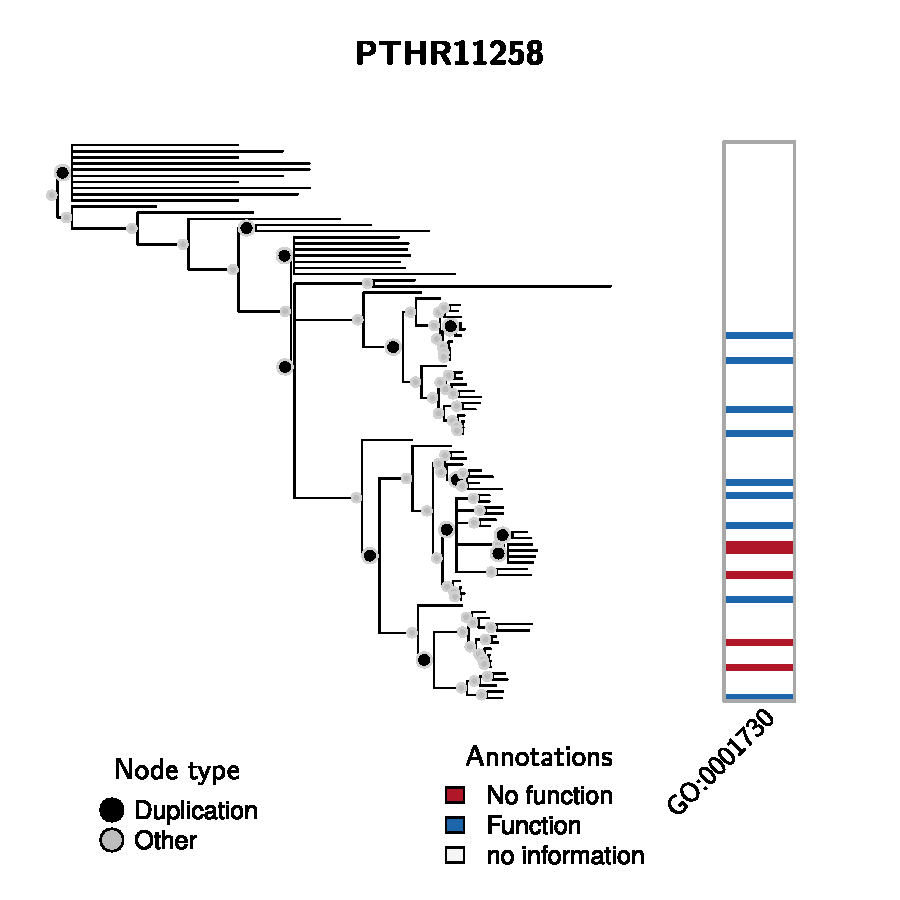
\includegraphics[width=.85\linewidth, clip, trim={0 0 0 1.5cm}]{example-trees-good1-parts-1.pdf}}%
			\only<2->{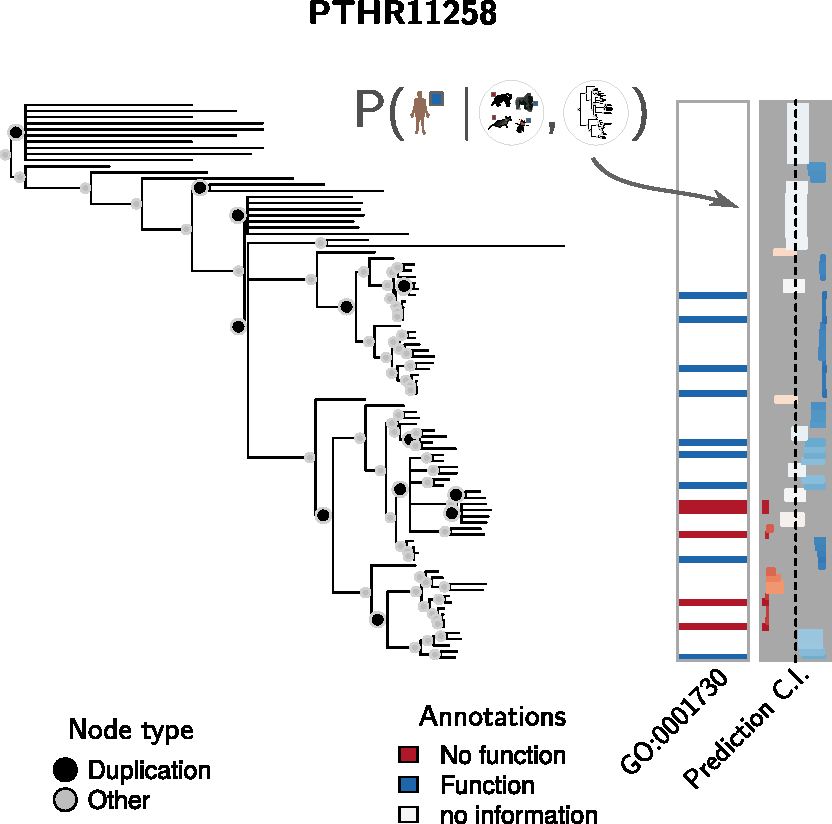
\includegraphics[width=.85\linewidth, clip, trim={0 0 0 1.5cm}]{example-trees-good1-parts-1b.pdf}}
		}
		\mode<handout>{
			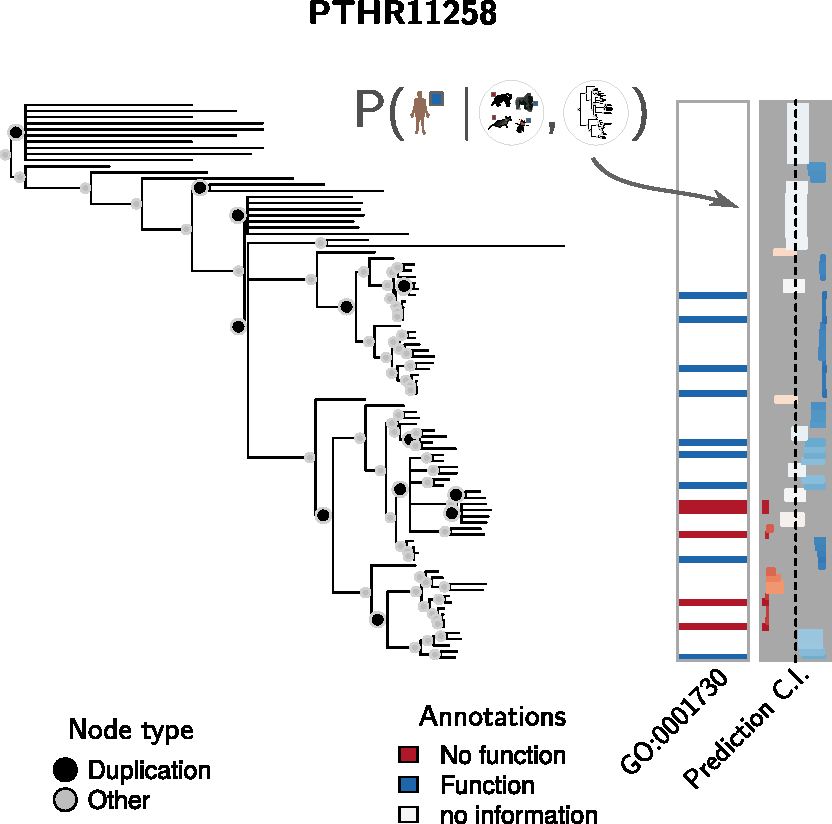
\includegraphics[width=.85\linewidth, clip, trim={0 0 0 1.5cm}]{example-trees-good1-parts-1b.pdf}
		}
	
		
	\end{minipage}
\end{frame}

%--------------------------------------------------------------------------------
\begin{frame}
	\frametitle{Computational features of \textbf{aphylo}}
	\begin{minipage}[m]{.55\linewidth}
		\vspace{-1cm}\raggedleft
\includegraphics[width=.35\linewidth]{aphylo-logo.png}\\\vspace{-.5cm}
		\raggedright
		\small
		\shadowbox{Baseline features}
		\begin{itemize}
			\item<2-> Parsimony: Conditional independence across functions/siblings.
			\item<3-> Post-order Tree traversal: Linear complexity $O(|\mbox{tree}|)$.
		\end{itemize}
		\uncover<4->{\shadowbox{Additional features}}
		\begin{itemize}
			\item<5-> Reduced pruning sequence: Induced sub-tree of nodes connected to annotated leafs\\ $\implies$ Complexity $O(\left|\mbox{Induced sub-tree}\right|)\leq O(|\mbox{tree}|)$
			\item<6-> Implemented in C++ (\textbf{pruner} library)
		\end{itemize}
	\end{minipage}\hfill
	\begin{minipage}[m]{.44\linewidth}
		\centering
		\uncover<5->{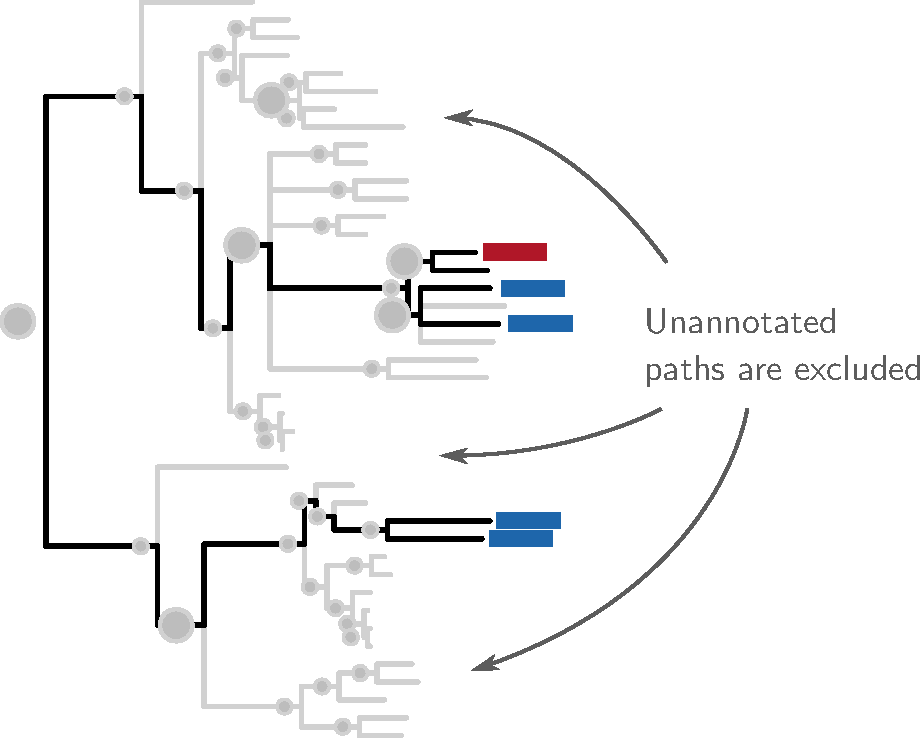
\includegraphics[width=1\linewidth]{reduced-sequence.pdf}}
	\end{minipage}
\end{frame}

% -------------------------------------------------------------------------------
\begin{frame}[c,label=aphylo-results-brief]
	\frametitle{Results: What does aphylo brings to the table?}
	\begin{center}
		
\includegraphics[width=.2\linewidth]{aphylo-logo.png}
	\end{center}
	
	\uncover<1->{\begin{minipage}[t]{.24\linewidth}\centering
			\shadowbox{Large scale}\\\small
			Estimate \textbf{pooled-data models} involving
			\textbf{hundreds of families}\\
			(1,300 genes at a time)
	\end{minipage}}\hfill
	\uncover<2->{\begin{minipage}[t]{.24\linewidth}\centering
			\shadowbox{Interpretable}\\\small
			Pooled-data model provides inference
			\textbf{aligned with theoretical results}\\
			(gene duplication is key)
	\end{minipage}}\hfill
	\uncover<3->{\begin{minipage}[t]{.24\linewidth}\centering
			\shadowbox{Fast}\\\small
			Computational efficiency
			allows making \textbf{inference and prediction fast}\\
			(1 second vs 2 hours)
	\end{minipage}}\hfill
	\uncover<4->{\begin{minipage}[t]{.24\linewidth}\centering
			\shadowbox{Accuracy}\\\small
			Outperforms state-of-the-art
			phylo-models\\
			(0.72 vs 0.60 AUC)
	\end{minipage}}
	\vfill\hfill\hyperlink{aphylo-results-overview}{\beamergotobutton{details}}
\end{frame}

% ------------------------------------------------------------------------------
\section{A general framework for modeling functional evolution}

\begin{frame}[t]
	\usebeamertemplate{section intro}{}{}
	\textcolor{uscgold}{
		\Large {\bf A general framework for modeling functional evolution} 
	}
\end{frame}


% ------------------------------------------------------------------------------
\begin{frame}[label=aphylo-current]
	\frametitle{Phylogenetics Modeling Strategies}
	
	\begin{minipage}[m]{.3\linewidth}
		
		\begin{figure}
			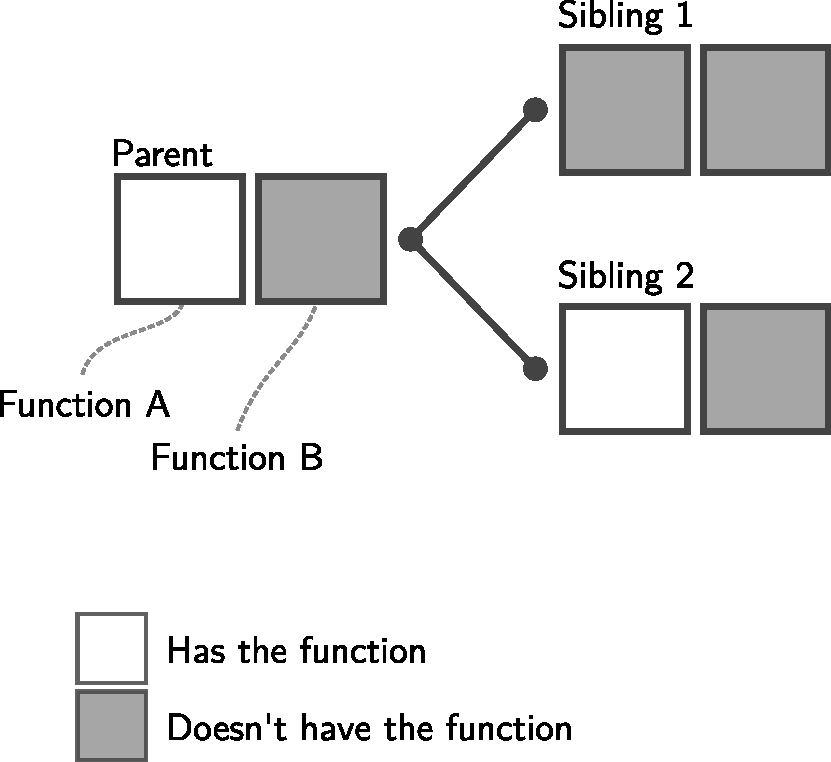
\includegraphics[width=.9\linewidth]{phylo-model-overview-legend.pdf}
		\end{figure}
		
		\uncover<5->{\large SNA could help us with\\\alert{\textbf{Exponential\\Random~Graph Models}}}
	\end{minipage}\hfill
	\begin{minipage}[m]{.69\linewidth}
		\mode<beamer>{
			\begin{figure}
				\phantom{\includegraphics<1>[width=.9\linewidth]{phylo-model-overview-1.pdf}}%
				\includegraphics<2>[width=.9\linewidth]{phylo-model-overview-1.pdf}%
				\includegraphics<3>[width=.9\linewidth]{phylo-model-overview-2.pdf}%
				\includegraphics<4>[width=.9\linewidth]{phylo-model-overview.pdf}
			\end{figure}
		}
		
		\mode<handout>{
			\begin{figure}
				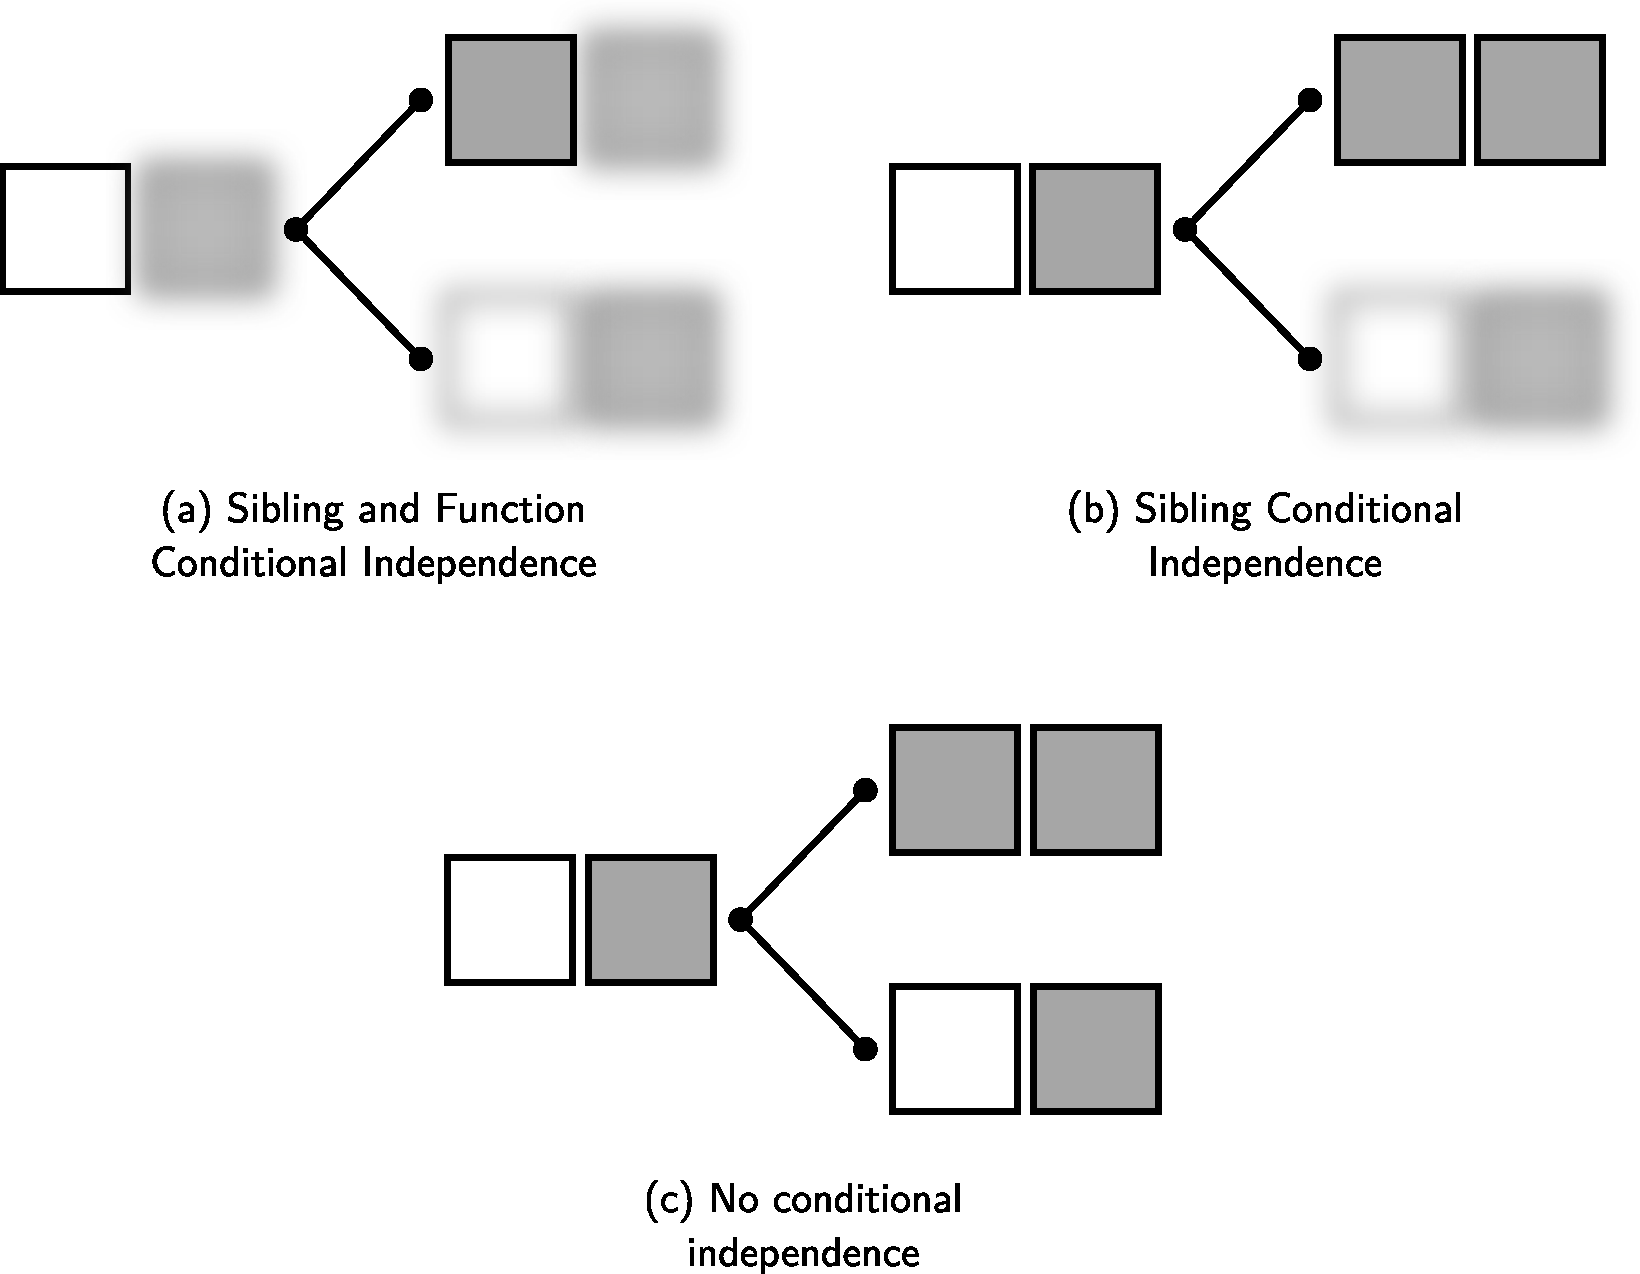
\includegraphics[width=.9\linewidth]{phylo-model-overview.pdf}
			\end{figure}
		}
	\end{minipage}
	
\end{frame}

%-------------------------------------------------------------------------------
\begin{frame}
	\frametitle{What are Exponential Random Graph Models}
	
	Exponential Family Random Graph Models, aka \alert{ERGMs} are:\pause
	
	\begin{itemize}
		\item Statistical models of (social) networks.\pause
		\item Social Network Analysis: What drives social connections?
		\item Not about individual ties, but about local structures (sufficient statistics).\pause
		\begin{figure}
			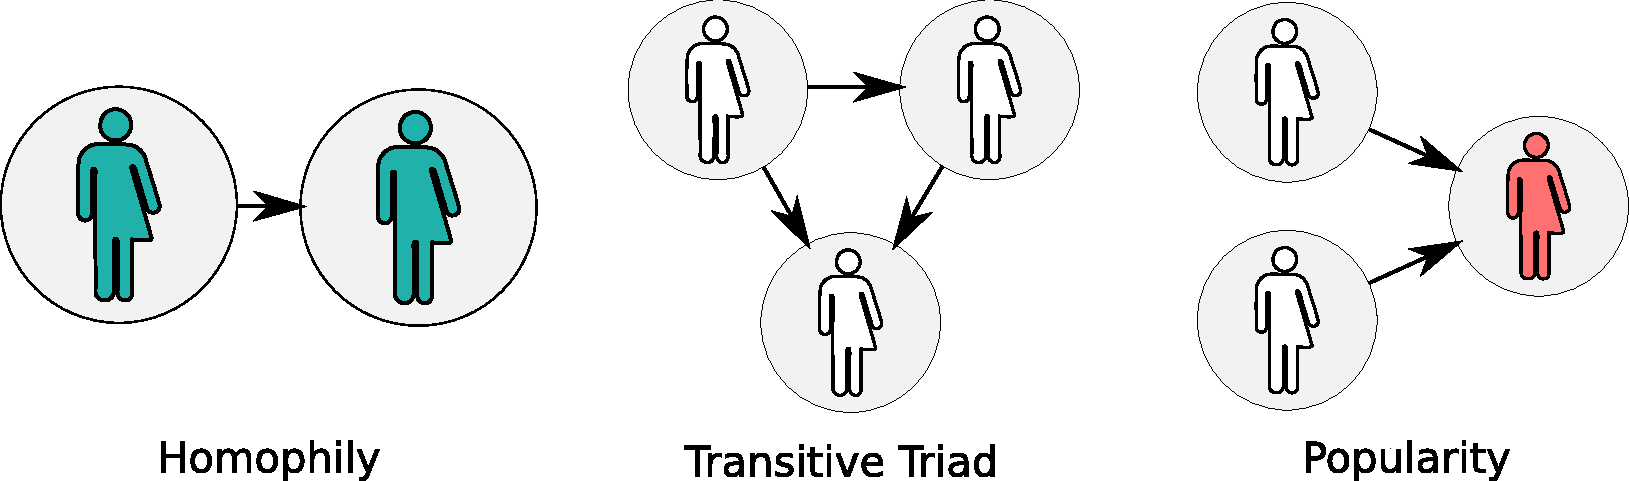
\includegraphics[width=.6\linewidth]{friendly-terms.pdf}
		\end{figure}
		\item Social Networks $\equiv$ Adjacency Matrix $\equiv$ Binary arrays
	\end{itemize}
	
\end{frame}

% -------------------------------------------------------------------------------
\begin{frame}
	\frametitle{Binary Arrays: A bridge between SNA and Phylogenetics}
	
	\begin{minipage}[c]{.49\linewidth}
	\begin{figure}
	    \centering
	    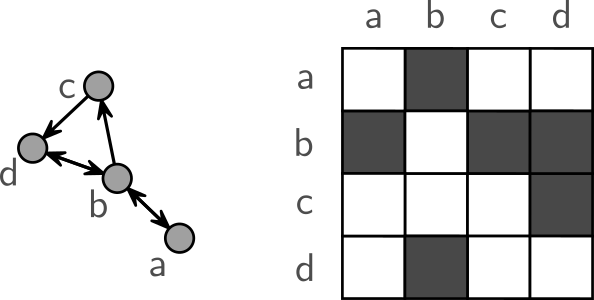
\includegraphics[width=.7\linewidth]{fig/adjmat-network.png}
	    \caption{Caption}
        \label{fig:my_label}
	\end{figure}    
	\end{minipage}\hfill
	\begin{minipage}[c]{.49\linewidth}
	\begin{figure}
	    \centering
	    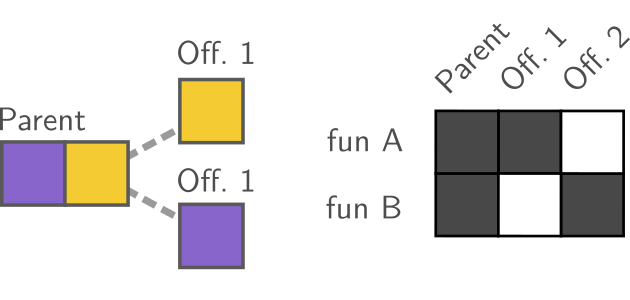
\includegraphics[width=.7\linewidth]{fig/adjmat-aphylo.png}
	    \caption{Caption}
        \label{fig:my_label}
	\end{figure}    
	\end{minipage}
	
\end{frame}

\begin{frame}
	\def\fwidth{.6\linewidth}
	\begin{table}
	\begin{tabular}{m{.2\linewidth}<\centering m{.2\linewidth}m{.4\linewidth}}
	\toprule
	Representation & Description & Definition  \\ \midrule
	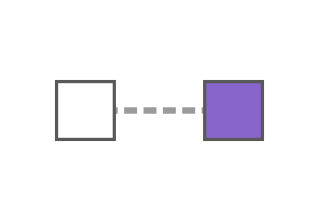
\includegraphics[width=\fwidth]{fig/term-gain.png} & %
		Gain of function & $(1 - x_p)\sum_{n:n\in Off}x_n$  \\
	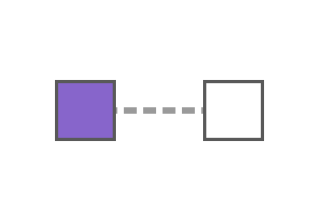
\includegraphics[width=\fwidth]{fig/term-loss.png} & %
		Loss of function & $x_p\sum_{n:n\in Off}(1 - x_n)$  \\
	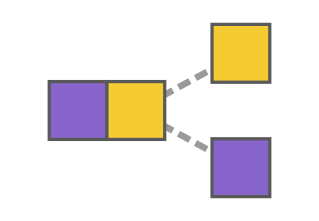
\includegraphics[width=\fwidth]{fig/term-subfun.png} & %
		Subfunctionalization & $x_p^kx_p^j\sum_{n\neq m}x_n^k(1-x_n^j)(1-x_m^k)x_m^j$  \\
	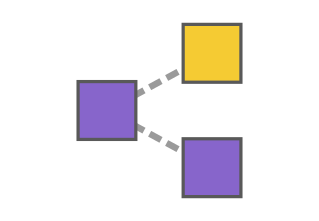
\includegraphics[width=\fwidth]{fig/term-neofun.png} & %
		Neofunctionalization & $x_p^k(1 - x_p^j)\sum_{n\neq m}x_n^k(1-x_n^j)(1-x_m^k)x_m^j$ \\
	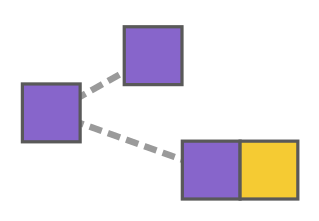
\includegraphics[width=\fwidth]{fig/term-longest.png} & %
		Longest branch gains & $(1-x_p^k)\isone{x_m^k : m=\mbox{argmax}_n\mbox{blength}_n}$ \\
	\bottomrule
	\end{tabular}
	\end{table}
\end{frame}



% ------------------------------------------------------------------------------
\begin{frame}[c,label=aphylo-ergm-example]
	
	\Large If we wanted to build a model with 3 functions, we would need to estimate...\large
	\\\bigskip
	
	\begin{minipage}[t]{.40\linewidth}
		\centering
		\shadowbox{Full Markov Transition Matrix}\\\bigskip
		\uncover<2->{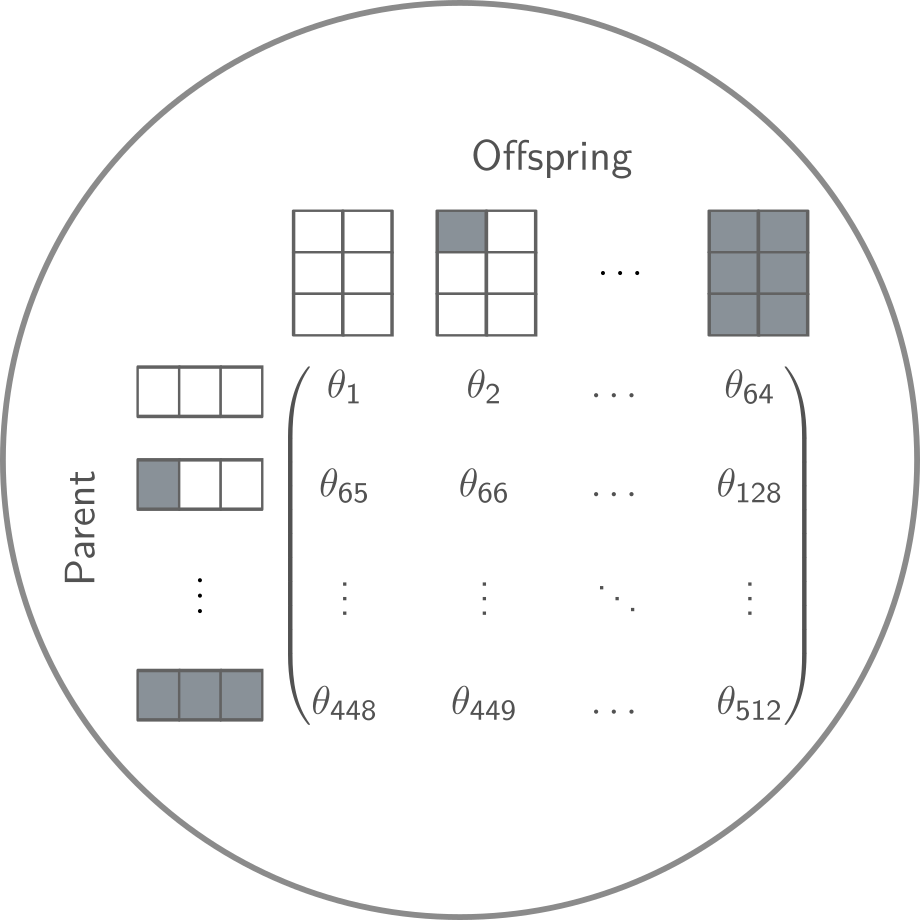
\includegraphics[width=.8\linewidth]{aphylo-ergm-eq1.png} \\
			\vfill 512 parameters
		}
	\end{minipage}\hfill
	\begin{minipage}[t]{.19\linewidth}
		\centering 
		\uncover<4->{
			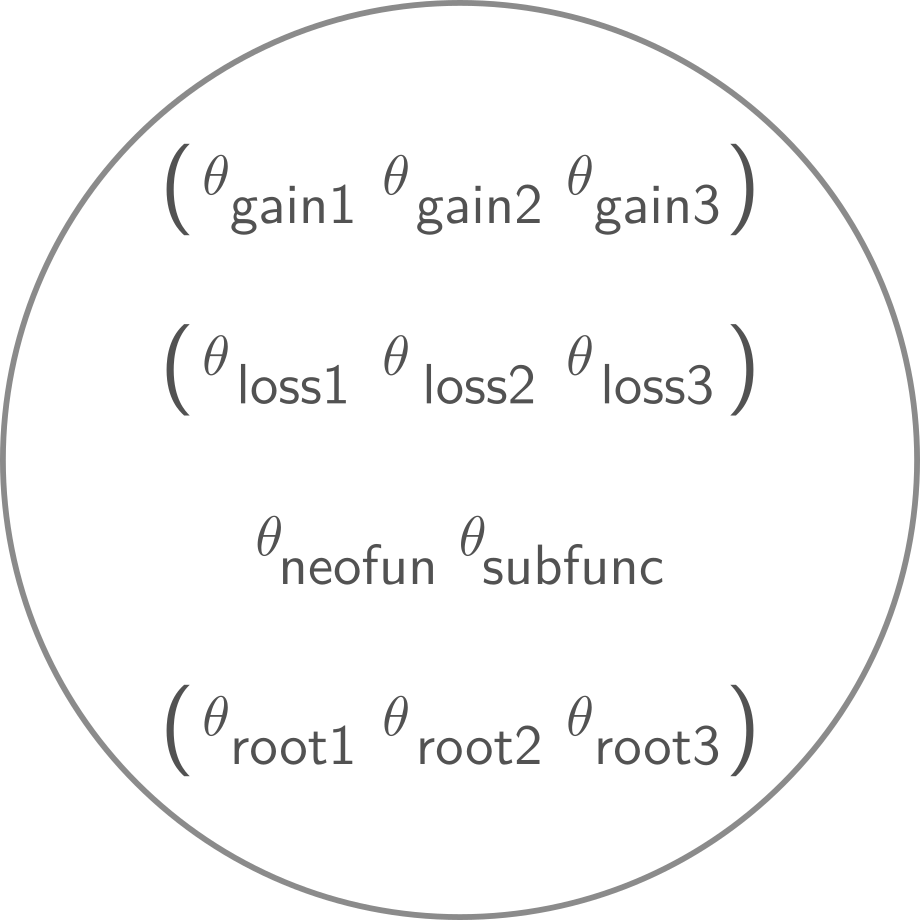
\includegraphics[width=.8\linewidth]{aphylo-ergm-eq2.png}\\
			Easier to fit \\
			Easier to interpret}	
	\end{minipage}\hfill
	\begin{minipage}[t]{.40\linewidth}		
		\centering
		\shadowbox{Sufficient statistics}\\\bigskip
		\uncover<3->{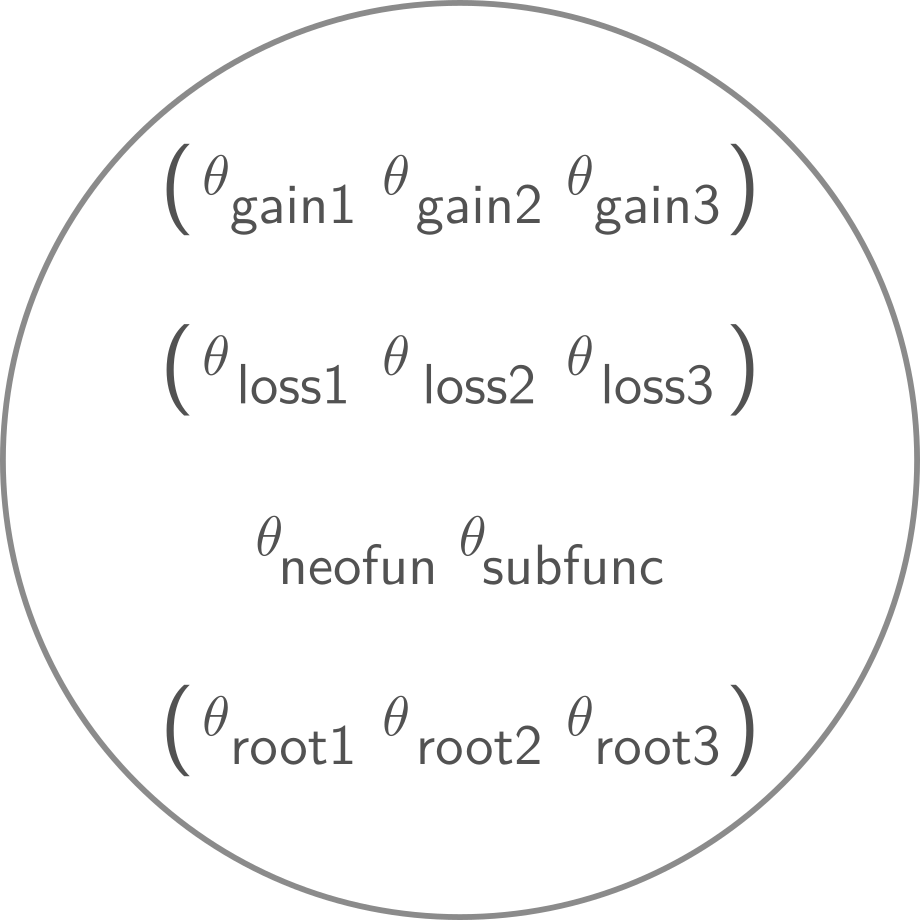
\includegraphics[width=.8\linewidth]{aphylo-ergm-eq2.png} \\
			\vfill 11 parameters}
	\end{minipage}
	\vfill
	\uncover<5->{...I implemented this (and more) in \textbf{barry}.}
	\uncover<4->{\hfill\hfill\hyperlink{current-research}{\beamerreturnbutton{numeric example}}}
\end{frame}

%-------------------------------------------------------------------------------
\begin{frame}[c]
	\centering
	
\includegraphics[width=.25\linewidth]{fig/barry-logo.png}
	
	\scalebox{1.5}{\bfseries\Huge{}{\color{usccardinal}Barr}\small{}a\Huge{}{\color{usccardinal}y}\normalsize}
	
	\scalebox{1.2}{C++ header-only library for counting structures in binary arrays}
	
	\pause
	\vfill\raggedright {\footnotesize \href{https://en.wikipedia.org/wiki/The_Sniffing_Accountant}{``The Sniffing Accountant'' (Seinfeld, Season 5, Episode 4)}}
\end{frame}

% -------------------------------------------------------------------------------
\begin{frame}
	\frametitle{Computational features of \textbf{barry}}
	\begin{minipage}[m]{.55\linewidth}
		\vspace{-1cm}\raggedleft
\includegraphics[width=.35\linewidth]{barry-logo.png}\\\vspace{-.5cm}
		\raggedright
		\small
		\shadowbox{Core}
		\begin{itemize}
			\item<2-> C++ header-only template library.
			\item<3-> Arrays $\equiv$ sparse matrices, i.e., small and large.
			\item<4-> Full enumeration and support of DEM.
			\item<5-> Arbitrary constrains for enumeration.
		\end{itemize}
		\uncover<6->{\shadowbox{Modeling features}}
		\begin{itemize}
			\item<7-> Arbitrary Model terms (suff. stats).
			\item<8-> Hashmap recycles support, i.e., pooled data models.
		\end{itemize}
	\end{minipage}\hfill
	\begin{minipage}[m]{.44\linewidth}
		\centering
		\uncover<8->{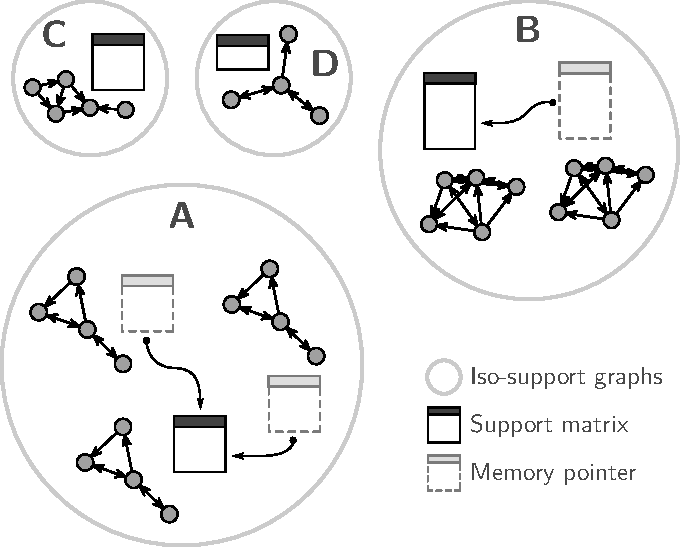
\includegraphics[width=1\linewidth]{ergm-computing.pdf}}
	\end{minipage}
\end{frame}

\begin{frame}[c]
	\frametitle{Example: Simple model with two functions}
	
\end{frame}


\begin{frame}[c]
	\frametitle{Example: Simple model with two functions}
	\framesubtitle{posterior distributions}
	\begin{figure}
	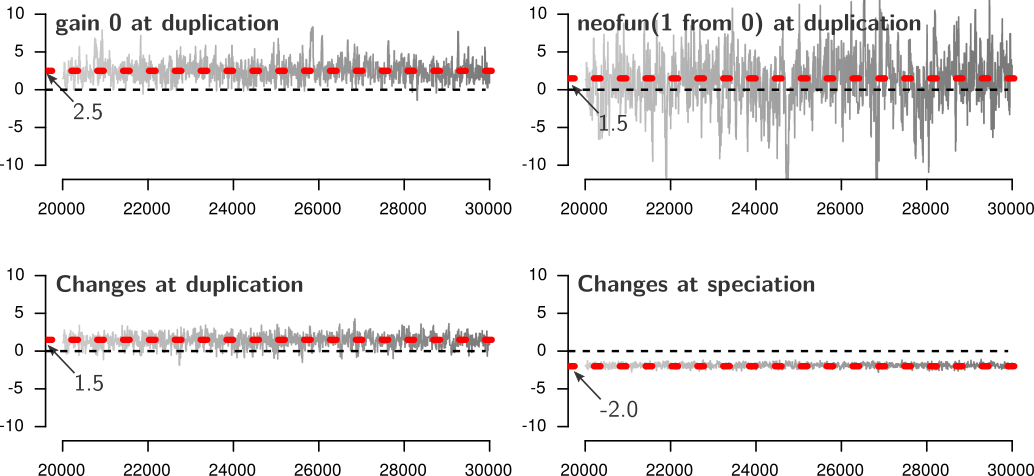
\includegraphics[width=.8\linewidth]{fig/trace-gain-neo.png}
	\caption{MCMC Trace of the functional gain of 0, neofunctionalization (1 from 0), and change rate (by event type). The true population parameters are:\linebreak$(\theta_{gain0}, \theta_{gain1}) = (2.0, 1.5)$ and $(\theta_{loss0}, \theta_{loss1}) = (-2.0, -1.5)$}
	\end{figure}
\end{frame}


\begin{frame}[c]
	\frametitle{Example: Simple model with two functions}
	\framesubtitle{posterior distributions (contd')}
	\begin{figure}
		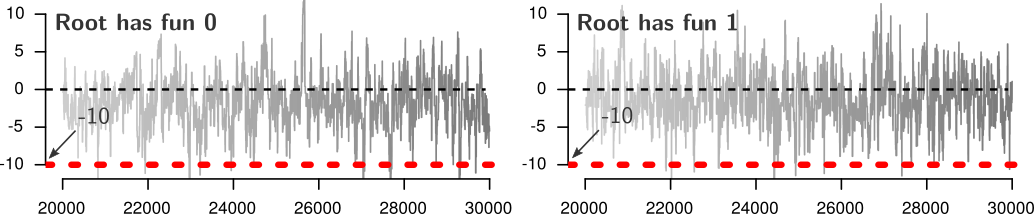
\includegraphics[width=.8\linewidth]{fig/trace-root.png}
		\caption{MCMC Trace of root parameters. The true population parameters are $(\theta_{root0}, \theta_{root1}) = (-10.0, -10.0)$}
	\end{figure}
\end{frame}


%-------------------------------------------------------------------------------
\begin{frame}
\frametitle{Simulation Study}

\begin{figure}
	\centering
		\caption{Distribution of parameter estimates from 5,000 annotated trees of size 99.
		Parameter estimates were obtained using MCMC with Robust Adaptive
		Metropolis and logistic prior with scale 2 and mean 0.
	}
	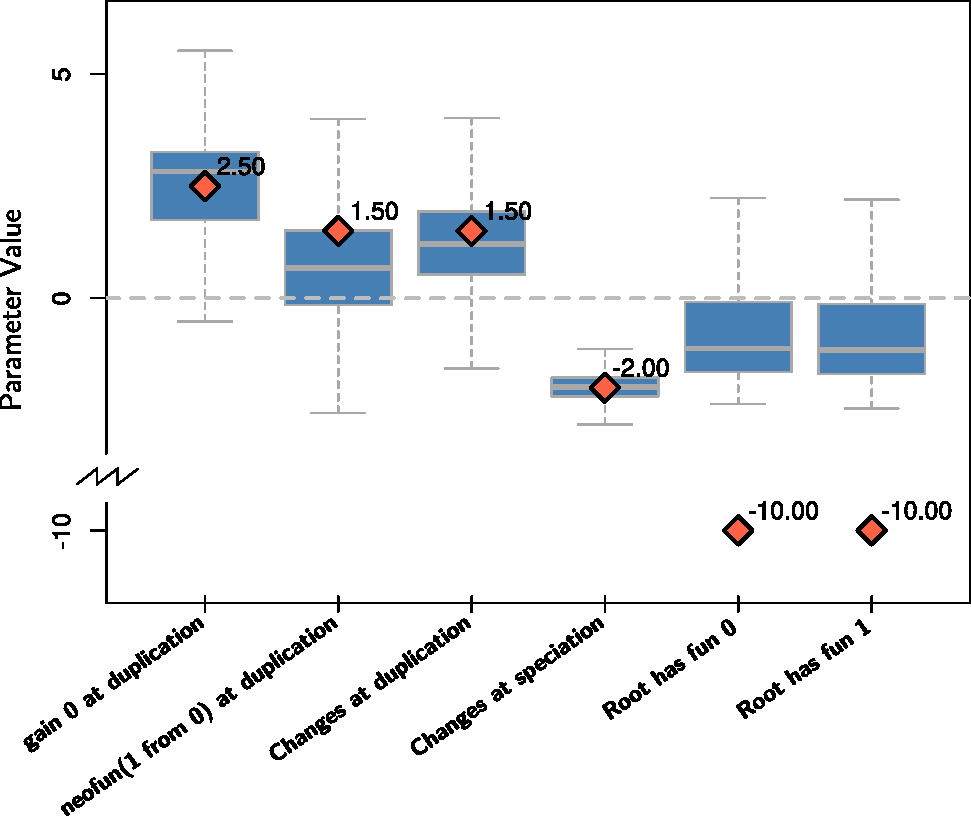
\includegraphics[width=.5\linewidth]{fig/aphylo-sim-study.pdf}
\end{figure}

\end{frame}
%-------------------------------------------------------------------------------
\begin{frame}
	
	\large The key lies in the \alert{transition probability}...\normalsize
	
	\begin{equation}
		\Prcond{\Ann=\mathbf{x}}{\ann{n}} = \frac{\exp{\t{\Theta} s(\mathbf{x},\ann{n})}}{\sum_{\mathbf{x}'}\exp{\t{\Theta} s(\mathbf{x}', \ann{n})}}
	\end{equation}
	where
	
	\begin{itemize}
	\item $\mathbf{x} \equiv \{\ann{n1}, \ann{n2},\dots\}$ is an array of size $P$ (functions) $\times$ $|\offspring{n}|$ (offspring)
	\item $\ann{n}$ is a binary vector (state of node $n$),
	\item $\Theta$ is a column vector of parameters, and
	\item $s(\cdot)$ is a column vector of sufficient statistics 
	\end{itemize}

It can be shown that the \alert{pruning} probability equals:
	
\begin{equation}
	\Prcond{\aphyloObs_n}{\mathbf{x}_{n}, \Theta} = %
	\sum_{\mathbf{x}}\Prcond{\mathbf{x}}{\mathbf{x}_{n}}\prod_{m \in \offspring{n}}\Prcond{\aphyloObs_{m}}{\mathbf{x}_{m}}\label{eq:depfun-depsibs}
\end{equation}
\end{frame}




%%-------------------------------------------------------------------------------
%\begin{frame}[c]
%	\centering
%	\mode<beamer>{\scalebox{1.5}{
%			\only<1>{barray}\only<2->{\Huge{}{\color{usccardinal}Barr}\small{}a\Huge{}{\color{usccardinal}y}\normalsize}:
%	}}\mode<handout>{\Huge{}{\color{usccardinal}Barr}\small{}a\Huge{}{\color{usccardinal}y}\normalsize}
%	
%	\scalebox{1.5}{C++ header-only library for counting structures in binary arrays}
%	\pause
%	\vfill\raggedright {\footnotesize \href{https://en.wikipedia.org/wiki/The_Sniffing_Accountant}{``The Sniffing Accountant'' (Seinfeld, Season 5, Episode 4)}}
%\end{frame}

% ------------------------------------------------------------------------------
%\newcommand{\ultima}[3]{\begin{minipage}[t]{#1\linewidth}%
%		\begin{center}\shadowbox{#2}\end{center}\vspace{-.55cm}\hfill%	
%
%		\small#3\normalsize\end{minipage}%
%	}
%\begin{frame}[t]
%\frametitle{Concluding Remarks}
%\small
%\pause
%\color<4->{gray}
%\ultima{.3}{Before my dissertation}{%
%	\textbf{Predicting gene functions}
%	\begin{itemize}
%		\item ``Small scale''.
%		\item Detached from theory.
%	\end{itemize}\pause
%	
%	\textbf{ERGMs}
%	\begin{itemize}
%		\item Only approximations.
%		\item Small networks overlooked.
%		\item Limited alternatives for small nets.
%	\end{itemize}\pause
%}\color<4->{black}\hfill
%\ultima{.3}{After my dissertation}{%
%	\textbf{Predicting gene functions}
%	\begin{itemize}
%		\item Scale-up the problem.
%		\item More biology (via ERGMs).
%		\item New ways to look at phylo data.
%	\end{itemize}\pause
%
%	\textbf{ERGMs}
%	\begin{itemize}
%		\item Revisited exact methods.
%		\item New light on small networks.
%		\item Many opportunities for methodological innovations.
%	\end{itemize}\pause
%
%	\vfill
%	
%
%}\hfill
%\ultima{.39}{Products}{
%\textbf{Publications}
%
%6 journal publications (\tiny Journal of Open Source Software, Stata Journal, Journal of health and social behavior, Translational behavioral medicine, Social Science \& Medicine\small)\pause\textbf{+2 submitted} (\tiny PLOS Comp. Bio, Social Networks\small)\pause
%
%\textbf{Published software}
%\begin{itemize}
%\item ergmito \includegraphics[width=.3\linewidth]{cran-downloads-ergmito.pdf}
%\item slurmR \includegraphics[width=.3\linewidth]{cran-downloads-slurmr.pdf}
%\item fmcmc \includegraphics[width=.3\linewidth]{cran-downloads-fmcmc.pdf}
%\item netdiffuseR \includegraphics[width=.3\linewidth]{cran-downloads-netdiffuser.pdf}
%\end{itemize}\pause
%
%\textbf{Other tools}\\
%similR, gnet, aphylo, polygons, pruner, netplot, rphyloxml, jsPhyloSVG,\pause{} and {\large\color{usccardinal}\textbf{Barry}}
%
%}
%
%\end{frame}

% ------------------------------------------------------------------------------
\begin{frame}[c]
	\centering
	\usebeamertemplate{section intro}{}{}
	\textbf{%
		\color{uscgold}
		\Large Triads, Dyads, and Gene Functions\\When Social Network Analysis Meets Phylogenetics\large %
	}

	\textbf{
		\color{uscgold}
		George G Vega Yon \\
		\url{https://ggvy.cl} \\
		vegayon@usc.edu
	}
	
	
\includemedia[%
	width=.3\linewidth,%
	height=.3\linewidth,%
	addresource=fig/walking-dead.mp4,%
	transparent,
	%transparent player background
	activate=pageopen,
	passcontext,
	%show VPlayer's right-click menu
	flashvars={
		source=fig/walking-dead.mp4
		&loop=true
		% loop video
	}
]{}{VPlayer.swf}
	
	
	\begin{center}
	\scalebox{2}{\textcolor{uscgold}{Thank you!}} 
	\end{center}
\end{frame}


\renewcommand{\section}[2]{}%
\appendix

% ------------------------------------------------------------------------------
% ------------------------------------------------------------------------------
% ------------------------------------------------------------------------------
% ------------------------------------------------------------------------------
% ------------------------------------------------------------------------------

% ------------------------------------------------------------------------------
\changemode{handout}

% ------------------------------------------------------------------------------
\begin{frame}[label=go-functions-types]
	\frametitle{Genes and their Functions}
	
	Gene functions can be classified in three types:
	
	\def\tmpwidth{.9\linewidth}
	
	\begin{table}
		\begin{tabular}{*{3}{m{.31\linewidth}<{\centering}}}
			\onslide<2->\bf Molecular function & %
			\onslide<3->\bf Cellular component & %
			\onslide<4->\bf Biological process \\
			\onslide<2->\href{http://amigo.geneontology.org/amigo/term/GO:0005215}{Active transport GO:0005215}& %
			\onslide<3->\href{http://amigo.geneontology.org/amigo/term/GO:0004016}{Mitochondria GO:0004016} & %
			\onslide<4->\href{http://amigo.geneontology.org/amigo/term/GO:0060047}{Heart contraction GO:0060047} \\
			\onslide<2->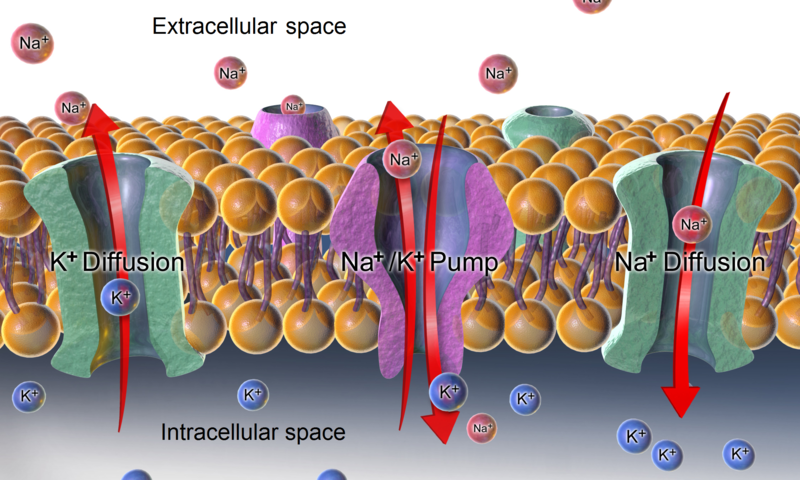
\includegraphics[width=\tmpwidth]{Sodium-potassium_pump_and_diffusion.png} & %
			\onslide<3->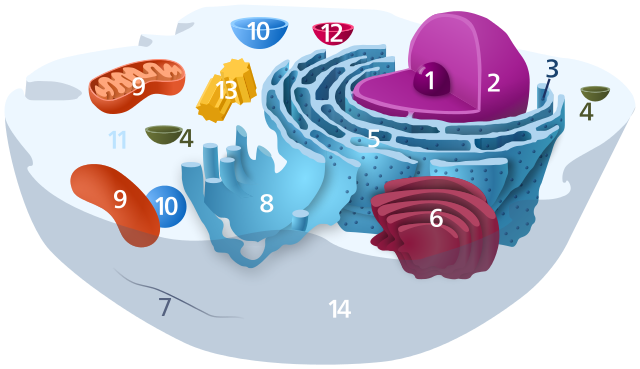
\includegraphics[width=\tmpwidth]{640px-Animal_Cell-svg.png} & % 
			\onslide<4->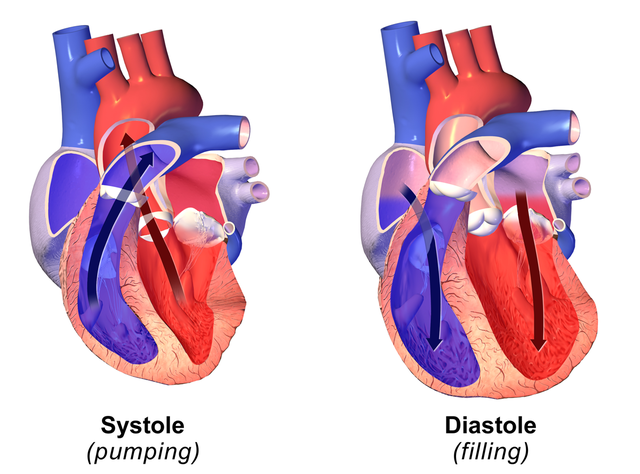
\includegraphics[width=\tmpwidth]{Systolevs_Diastole.png}
		\end{tabular}
	\end{table}
	
	\vfill \hfill \hyperlink{geneontology}{\beamerreturnbutton{go back}}
	
\end{frame}


\begin{frame}[label=aphylo-goexample]
\frametitle{The Gene Ontology Project}

Example of GO term

\begin{table}
\footnotesize
\begin{tabular}{lm{.6\linewidth}}
\toprule
\textbf{Accession} & GO:0060047 \\
\textbf{Name} & heart contraction \\
\textbf{Ontology} & biological\_process \\
\textbf{Synonyms} & heart beating, cardiac contraction, hemolymph circulation \\
\textbf{Alternate} & IDs None \\
\textbf{Definition} & The multicellular organismal process in which the heart decreases in volume in a 
characteristic way to propel blood through the body. Source: GOC:dph \\
\bottomrule
\end{tabular}
\caption{Heart Contraction Function. source: \href{http://amigo.geneontology.org/amigo/term/GO:0060047}{amigo.geneontology.org}}
\end{table}%\pause

You know what is interesting about this function?

\vfill \hfill \hyperlink{geneontology}{\beamerreturnbutton{go back}}

\end{frame}

% ------------------------------------------------------------------------------
\begin{frame}[t]

These four species have a gene with that function... \uncover<2->{and two of %
these are part of the same evolutionary tree!}

\vfill

\def\tmpwidth{.30\linewidth}
\begin{table}
\footnotesize
\mode<beamer>{
\begin{tabular}{*{2}{m{\tmpwidth}<\centering}}
\only<1>{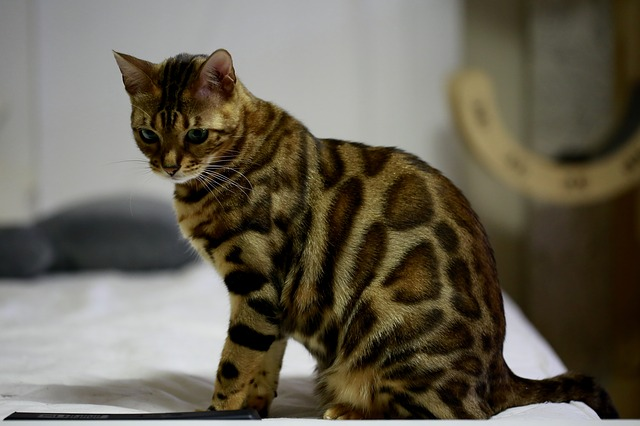
\includegraphics[width=.95\linewidth]{cat.jpg}} %
  \only<2->{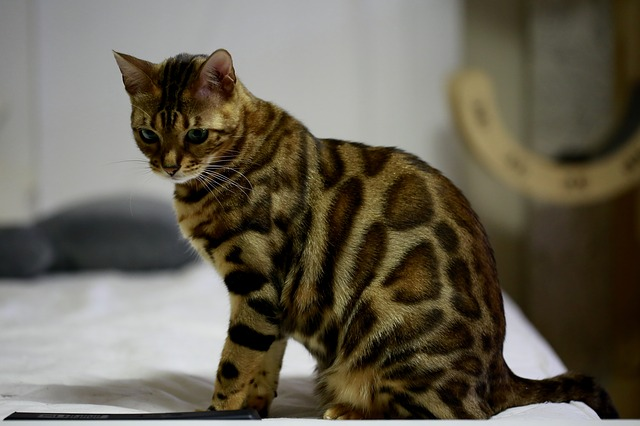
\includegraphics[width=.4\linewidth]{cat.jpg}} \linebreak Felis catus pthr10037 & %
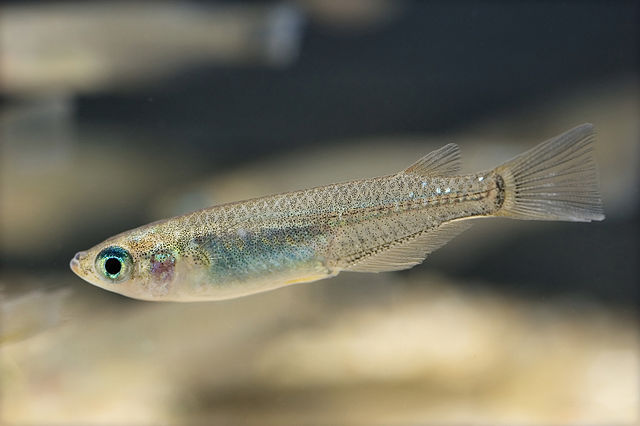
\includegraphics[width=1\linewidth]{Oryzias_latipes.jpg} \linebreak Oryzias latipes \textbf{pthr11521} \\ %
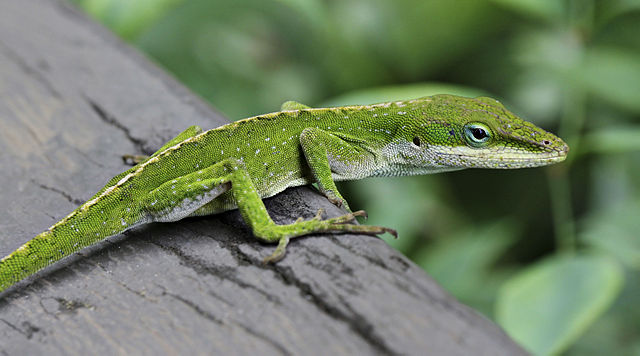
\includegraphics[width=1\linewidth]{Anole_Lizard.jpg} \linebreak Anolis carolinensis \textbf{pthr11521} & %
\only<1>{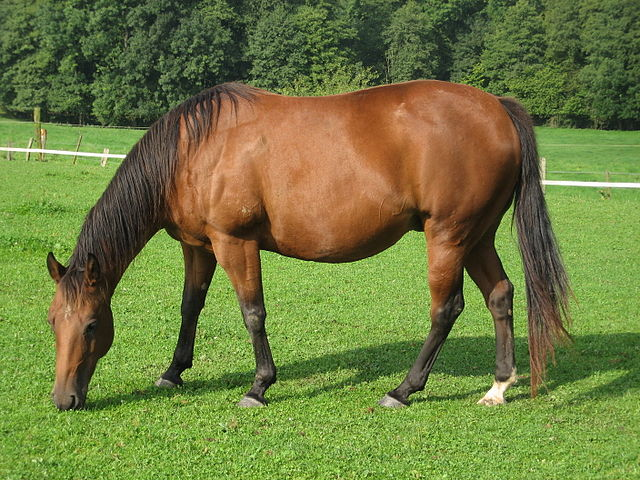
\includegraphics[width=.725\linewidth]{horse.jpg}} %
  \only<2->{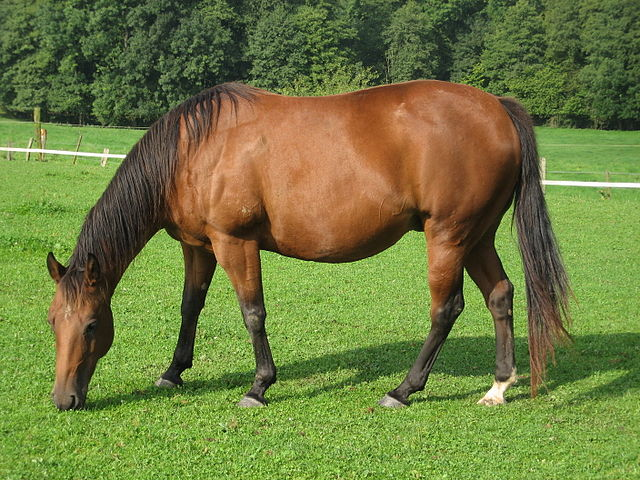
\includegraphics[width=.4\linewidth]{horse.jpg}} \linebreak Equus caballus pthr24356
\end{tabular}
}
\mode<handout>{
	\begin{tabular}{*{2}{m{\tmpwidth}<\centering}}
		\includegraphics[width=.4\linewidth]{cat.jpg} \linebreak Felis catus pthr10037 & %
		\includegraphics[width=1\linewidth]{Oryzias_latipes.jpg} \linebreak Oryzias latipes \textbf{pthr11521} \\ %
		\includegraphics[width=1\linewidth]{Anole_Lizard.jpg} \linebreak Anolis carolinensis \textbf{pthr11521} & %
		\includegraphics[width=.4\linewidth]{horse.jpg} \linebreak Equus caballus pthr24356
	\end{tabular}
}
\end{table}

\vfill \hfill \hyperlink{geneontology}{\beamerreturnbutton{go back}}

\end{frame}

%--------------------------------------------------------------------------------
%\newcommand{\oinclude}[2]{\only<#1>{\includegraphics[width=\tmpwdth,clip,trim={0 0 0 2cm}]{#2}}}

\begin{frame}[t, label=aphylo-good-details]
	\frametitle{Example of Data + Predictions}
	
	\begin{minipage}[m]{.3\linewidth}
		\small
		%	The AUC for this analysis is 0.91 and the Mean Absolute Error is 0.34
		\uncover<1->{\textbf{Family: PTHR11258}}\\
		\uncover<1->{%
			\textbf{Type:} Molecular Function\\
			\textbf{Name:} 2'-5'-oligoadenylate synthetase activity\\
			\textbf{Desc:}  \href{http://amigo.geneontology.org/amigo/term/GO:0001730}{\alert{GO:0001730}} involved in the process of cellular antiviral activity (wiki on \href{https://en.wikipedia.org/wiki/Interferon}{\alert{interferon}}).
		}\\
		\uncover<2->{%
			\textbf{MAE:} 0.34 \\
			\textbf{AUC:} 0.91%
		}
		\vfill
		\hyperlink{aphylo-bad}{\beamerbutton{see a bad one}} 
		\hyperlink{aphylo-good}{\beamerreturnbutton{go back}}
	\end{minipage}
	\begin{minipage}[m]{.65\linewidth}
		\def\tmpwdth{.9\linewidth}
		\mode<beamer>{
			\centering
			\oinclude{1}{example-trees-good1-loo-annotated-parts-1.pdf}%
			\oinclude{2}{example-trees-good1-loo-annotated-0.pdf}%
			\oinclude{3}{example-trees-good1-loo-annotated-1.pdf}%
			\oinclude{4}{example-trees-good1-loo-annotated-2.pdf}%
			\oinclude{5}{example-trees-good1-loo-annotated.pdf}
			%			\only<1>{\includegraphics[width=\tmpwdth, clip, trim={0 0 0 2cm}]{example-trees-good1-loo-annotated-0.pdf}}\only<2>{\includegraphics[width=\tmpwdth, clip, trim={0 0 0 2cm}]{example-trees-good1-loo-annotated-1.pdf}}\only<3>{\includegraphics[width=\tmpwdth, clip, trim={0 0 0 2cm}]{example-trees-good1-loo-annotated-2.pdf}}\only<4>{\includegraphics[width=\tmpwdth, clip, trim={0 0 0 2cm}]{example-trees-good1-loo-annotated.pdf}}
		}
		
		\mode<handout>{
			\centering
			\includegraphics[width=\tmpwdth, clip, trim={0 0 0 2cm}]{example-trees-good1-loo-annotated.pdf}
		}
		
	\end{minipage}
\end{frame}

\begin{frame}[t,label=aphylo-bad]
	\frametitle{Example 2: Bad quality prediction}
	
	\begin{minipage}[m]{.3\linewidth}
		\small
		%	The AUC for this analysis is 0.91 and the Mean Absolute Error is 0.34
		\textbf{MAE:} 0.52 \\
		\textbf{AUC:} 0.33 \\
		\textbf{Type:} Molecular Function\\
		\textbf{Name:} mannosyl-oligosaccharide 1,2-alpha-mannosidase activity\\
		\textbf{Desc:}  \href{http://amigo.geneontology.org/amigo/term/GO:0004571}{\alert{GO:0004571}} involved in synthesis of glycoproteins (\href{https://en.wikipedia.org/wiki/Mannosyl-oligosaccharide_1,2-alpha-mannosidase}{\alert{wiki}} and \href{https://en.wikipedia.org/wiki/Glycoprotein}{\alert{examples}}).
		
		\hyperlink{aphylo-good}{\beamerreturnbutton{go back}}
	\end{minipage}
	\begin{minipage}[m]{.65\linewidth}
		\def\tmpwdth{.9\linewidth}
		\mode<beamer>{
			\centering
			\only<1>{\includegraphics[width=\tmpwdth, clip, trim={0 0 0 2cm}]{example-trees-bad1-loo-annotated-0.pdf}}\only<2>{\includegraphics[width=\tmpwdth, clip, trim={0 0 0 2cm}]{example-trees-bad1-loo-annotated-1.pdf}}\only<3>{\includegraphics[width=\tmpwdth, clip, trim={0 0 0 2cm}]{example-trees-bad1-loo-annotated.pdf}}
		}
		
		\mode<handout>{
			\centering
			\includegraphics[width=\tmpwdth, clip, trim={0 0 0 2cm}]{example-trees-bad1-loo-annotated.pdf}
		}
		
	\end{minipage}
	
	
\end{frame}



% --------------------------
\begin{frame}[label=aphylo-pooled]

% latex table generated in R 3.6.3 by xtable 1.8-4 package
% Tue Apr 28 11:51:17 2020
\begin{table}[tb]
	\centering
	\begin{tabular}{m{.14\linewidth}*{3}{m{.14\linewidth}<\centering}}
		\toprule & \multicolumn{1}{c}{\textit{Pooled-data}} & \multicolumn{2}{c}{One-at-a-time} \\ \cmidrule(r){2-2}\cmidrule(r){3-4}
		& Beta prior & Unif. prior & Beta Prior \\ 
		\midrule
		\textit{Pooled-data} \\
		\hspace{2mm}Unif. prior & \cellcolor{blue!25}[-0.02,-0.01] & \cellcolor{blue!25}[-0.14,-0.10] & \cellcolor{blue!25}[-0.06,-0.03] \\ 
		\hspace{2mm}Beta prior &  - & \cellcolor{blue!25}[-0.12,-0.09] & \cellcolor{blue!25}[-0.04,-0.01] \\ 
		\textit{One-at-a-time} \\
		\hspace{2mm}Unif. prior &  - & - & \cellcolor{red!25}[\hphantom{-}0.06,\hphantom{-}0.09] \\ 
		\bottomrule
	\end{tabular}
	\caption[Differences in Mean Absolute Error]{Differences in Mean Absolute Error [MAE]. Each cell shows the 95\% confidence interval for the difference in MAE resulting from two methods (row method minus column method). Cells are color coded blue when the method on that row has a significantly smaller MAE than the method on that column; Conversely, cells are colored red when the method in that column outperforms the method in that row.  Overall, predictions calculated using the parameter estimates from \textit{pooled-data} predictions outperform \textit{one-at-a-time}.}
	\label{tab:vs-accuracy}
\end{table}

\end{frame}


% ------------------------------------------------------------------------------
\begin{frame}[label = duplicationvsspeciation]
\frametitle{Speciation}
\begin{figure}
\centering
\def\svgwidth{.8\linewidth}
\tiny
% Source 
\input{fig/Drosophila_speciation_experiment.pdf_tex}
\caption{Dodd (1989): After one year of isolation, flies showed a significant level of assortativity in mating (\href{https://commons.wikimedia.org/wiki/File:Drosophila_speciation_experiment.svg}{wikimedia})}
\end{figure}

\vfill\hfill \hyperlink{aphylographicalview}{\beamerreturnbutton{go back}}

\end{frame}

\begin{frame}
\frametitle{Duplication}
\begin{figure}
\centering
\def\svgwidth{.6\linewidth}
\tiny
% Source : https://en.wikipedia.org/wiki/File:Evolution_fate_duplicate_genes_-_vector.svg
\input{fig/Evolution_fate_duplicate_genes_-_vector.pdf_tex}
\caption{A key part of molecular innovation, gene duplication provides opportunity for new functions to emerge (\href{https://en.wikipedia.org/wiki/File:Evolution_fate_duplicate_genes_-_vector.svg}{wikimedia})}
\end{figure}

\vfill\hfill \hyperlink{aphylographicalview}{\beamerreturnbutton{go back}}

\end{frame}

% ------------------------------------------------------------------------------
\begin{frame}[label=aphylo-data]
	\frametitle{Data: Phylogenetic trees}
	
	Sample of annotations (first 10 in a single tree, Phosphoserine Phosphatase [PTHR10000])
	
	\small
	
	\begin{table}[ht]
		\centering
		\begin{tabular}{rrll}
			\toprule
			Internal id & Branch Length & type & ancestor \\ 
			\midrule
			AN0 &  & S & LUCA \\ 
			AN1 & 0.06 & S & Archaea-Eukaryota \\ 
			AN2 & 0.24 & S & Eukaryota \\ 
			AN3 & 0.44 & S & Unikonts \\ 
			AN4 & 0.42 & S & Opisthokonts \\ 
			AN6 & 0.68 & D &  \\ 
			AN9 & 0.79 & S & Amoebozoa \\ 
			AN10 & 0.18 & D &  \\ 
			AN15 & 0.57 & S & Dictyostelium \\ 
			AN18 & 0.52 & S & Alveolata-Stramenopiles \\ 
			\bottomrule
		\end{tabular}
	\end{table}
	\vfill\hfill\hyperlink{phylo-table}{\beamerreturnbutton{go back}}
\end{frame}

\begin{frame}
	\frametitle{Data: Node type (events)}
	\begin{figure}
		\centering
		\includegraphics[width=.7\linewidth]{distribution-event-type.pdf}
	\end{figure}
	\vfill\hfill\hyperlink{phylo-table}{\beamerreturnbutton{go back}}
\end{frame}

\begin{frame}
	\frametitle{Data: Annotations (example)}
	
	This is the first 10 of $\sim$ 400,000 experimental annotations used:
	
	\footnotesize
	\begin{table}[ht]
		\centering
		\begin{tabular}{rllll}
			\toprule
			& Family & Id & GO term & Qualifier \\ 
			\midrule
			1 & PTHR12345 & HUMAN$|$HGNC=15756$|$UniProtKB=Q9H190 & GO:0005546 &  \\ 
			2 & PTHR11361 & HUMAN$|$HGNC=7325$|$UniProtKB=P43246 & GO:0016887 & CONTRIBUTES\_TO \\ 
			3 & PTHR10782 & MOUSE$|$MGI=MGI=3040693$|$UniProtKB=Q6P1E1 & GO:0045582 &  \\ 
			4 & PTHR23086 & ARATH$|$TAIR=AT3G09920$|$UniProtKB=Q8L850 & GO:0006520 &  \\ 
			5 & PTHR32061 & RAT$|$RGD=619819$|$UniProtKB=Q9EPI6 & GO:0043197 &  \\ 
			6 & PTHR46870 & ARATH$|$TAIR=AT3G46870$|$UniProtKB=Q9STF9 & GO:1990825 &  \\ 
			7 & PTHR15204 & MOUSE$|$MGI=MGI=1919439$|$UniProtKB=Q9Z1R2 & GO:0045861 &  \\ 
			8 & PTHR22928 & DROME$|$FlyBase=FBgn0050085$|$UniProtKB=Q9XZ34 & GO:0030174 &  \\ 
			9 & PTHR35972 & HUMAN$|$HGNC=34401$|$UniProtKB=A2RU48 & GO:0005515 &  \\ 
			10 & PTHR10133 & DROME$|$FlyBase=FBgn0002905$|$UniProtKB=O18475 & GO:0097681 &  \\ 
			\bottomrule
		\end{tabular}
	\end{table}
	\vfill\hfill\hyperlink{phylo-table}{\beamerreturnbutton{go back}}
\end{frame}

\begin{frame}
	\frametitle{Data: Experimental Annotations}
	\begin{figure}
		\centering
		\includegraphics[width=.7\linewidth]{distribution-annotation-type.pdf}
	\end{figure}
	\vfill\hfill\hyperlink{phylo-table}{\beamerreturnbutton{go back}}
\end{frame}

\begin{frame}[label=aphylo-results-overview]
	\frametitle{Results: Implementation and Large scale study}
	
	\begin{minipage}[m]{.69\linewidth}
		\begin{itemize}
			\item<1-> Simulation, estimation, and prediction: \textbf{aphylo} R package.
			\item<2-> Large simulation study (all known trees, about 15,000) on USC's HPC cluster.
			\item<3-> Prediction quality assessment on $\sim$ 1,300 genes involving $\sim$ 130 families...
			estimation of parameters using a pooled-data model ($<$ 5 min). \hyperlink{aphylo-model-levels}{\beamerreturnbutton{modeling}} \hyperlink{aphylo-table}{\beamerreturnbutton{estimates}}
			\item<4-> In a subset of $\sim 200$ predictions we found 46 novel annotations 
			\hyperlink{aphylo-200funs}{\beamergotobutton{more}}
		\end{itemize}
	\end{minipage}\hfill
	\begin{minipage}[m]{.3\linewidth}
		\begin{center}
			\includegraphics[width=.9\linewidth]{aphylo-logo.png}
		\end{center}
	\end{minipage}
	
	\vfill\hfill\hyperlink{aphylo-results-brief}{\beamerreturnbutton{go back}}
	
\end{frame}

\begin{frame}[c]
	\frametitle{Results: Performance and Scalability}
	aphylo vs SIFTER (state-of-the-art phylo-based model) on 147 genes.
	
	\begin{minipage}[m]{.50\linewidth}
		\bigskip
		\uncover<3->{\begin{figure}
				\includegraphics[width=1\linewidth]{auc.pdf}
		\end{figure}}
	\end{minipage}\hfill
	\begin{minipage}[m]{.45\linewidth}
		\bigskip
		\begin{itemize}
			\item<2->[] \shadowbox{Fast} 110 minutes (SIFTER) to calculate the posterior probabilities, aphylo took 1 second.
			\item<3->[] \shadowbox{Accurate} aphylo reported higher accuracy levels in LOO cross-validation (0.72 vs 0.60 AUC).
		\end{itemize}
	\end{minipage}
	
\end{frame}


% ------------------------------------------------------------------------------
% ------------------------------------------------------------------------------
% ------------------------------------------------------------------------------
% ------------------------------------------------------------------------------


\begin{frame}[c,label=aphylo-table]
	\frametitle{Overview of Prediction Results}
	
	\begin{minipage}[m]{.55\linewidth}
		\begin{table}
			\centering
			\scalebox{.64}{
				\begin{tabular}{%
						m{.24\linewidth}<\raggedright %
						>{\color<1>{usccardinal}}m{.24\linewidth}<\centering%
						>{\color<2>{usccardinal}}m{.24\linewidth}<\centering%
						>{\color<3>{usccardinal}}m{.24\linewidth}<\centering%
						>{\color<4>{usccardinal}}m{.24\linewidth}<\centering}
					\toprule
					& & \multicolumn{3}{c}{Type of Annotation} \\
					\cmidrule(r){3-5} %
					\phantom{\LARGE Cellular Component}& %
					\alt<1>{\LARGE Pooled}{Pooled} & %
					\alt<2>{\LARGE Molecular Function}{Molecular Function} & %
					\alt<3>{\LARGE Biological Process}{Biological Process} & %
					\alt<4>{\LARGE Cellular Comp.}{Cellular Component} \\ 
					\midrule
					\multicolumn{3}{l}{\hspace{-10pt}Mislabeling} \\
					$\psi_{01}$ & 0.23 & 0.18 & 0.09 & \multirow{11}{*}{\uncover<4->{\Huge ?}}\\ %0.66 \\ 
					$\psi_{10}$ & 0.01 & 0.01 & 0.01 & \\ %0.33 \\ 
					\multicolumn{3}{l}{\hspace{-10pt}Duplication Events} \\
					$\mu_{d01}$ & 0.97 & 0.97 & \hlcAlt{3}{0.10} & \\ %0.55 \\ 
					$\mu_{d10}$ & 0.52 & 0.51 & \hlcAlt{3}{0.03} & \\ %0.56 \\ 
					\multicolumn{3}{l}{\hspace{-10pt}Speciation Events} \\
					$\mu_{s01}$ & 0.05 & 0.05 & 0.05 & \\ % 0.37 \\ 
					$\mu_{s10}$ & 0.01 & 0.01 & 0.02 & \\ % 0.37 \\ 
					\multicolumn{3}{l}{\hspace{-10pt}Root node} \\
					$\pi$ & 0.79 & 0.71 & 0.88 & \\ %0.52 \\ \midrule
					Trees & 141 & 74 & 45 & 22 \\ 
					\multicolumn{3}{l}{\hspace{-10pt}Accuracy under the by-aspect model} \\
					AUC & - & \hlcAlt{2}{0.77} & \hlcAlt{3}{0.83} & \\ % 0.53 \\ 
					MAE & - & \hlcAlt{2}{0.34} & \hlcAlt{3}{0.26} & \\ % 0.50 \\ 
					\multicolumn{3}{l}{\hspace{-10pt}Accuracy under the pooled-data model} \\
					AUC & - & \hlcAlt{2}{0.77} & 0.75 & \\ % 0.75 \\ 
					MAE & - & \hlcAlt{2}{0.35} & 0.34 & \\ %0.37 \\ 
					\bottomrule
			\end{tabular}}
			%\caption[Parameter estimates comparing pooled-data vs by-type]{MCMC estimates for experimentally annotated trees. The first column shows the estimates under the pooled-data model in \ref{tab:pooled-experimentally-annotated}, while the following three columns report the estimates obtained when fitting the model using a pooled-data approach, but doing so by type of annotation. Readers should be aware that the estimation process of the fourth column, \textit{cellular component}, did not fully converge, likely due to sparsity of annotations within that category.}
			\label{tab:by-aspect-estimates}
		\end{table}
	\end{minipage}
	\hfill
	\begin{minipage}[m]{.44\linewidth}
		Previously, joint estimates out-performed one-at-a-time\pause
		\begin{itemize}
			\item \textbf{Molecular Function} No change.\pause
			\item \textbf{Biological Process} Significantly better.\pause
			\item \textbf{Cellular Component} Does not converge.\pause
		\end{itemize}
		
		
		
		\small
		\begin{table}
			\begin{tabular}{%
					m{.22\linewidth}<\centering m{.03\linewidth}<\centering%
					m{.22\linewidth}<\centering m{.03\linewidth}<\centering%
					m{.25\linewidth}<\centering%
				}
				Molecular Function & $\neq$ & Biological Process &  ? & Cellular Component
			\end{tabular}
		\end{table}
		\normalsize
		
		\only<1->{\vfill\hfill\hyperlink{aphylo-data}{\beamergotobutton{data}}}
		\only<1->{\vfill\hfill\hyperlink{aphylo-results-overview}{\beamergotobutton{go back}}}
		
	\end{minipage}
	
	
	
\end{frame}

\begin{frame}[c,label=aphylo-200funs]
	\begin{figure}
		\includegraphics[width=.6\linewidth]{aphylo-results.pdf}
		\caption{Distribution of predictions}
	\end{figure}
	\vfill\hfill\hyperlink{aphylo-results-overview}{\beamerreturnbutton{go back}}
\end{frame}





% ------------------------------------------------------------------------------
\begin{frame}[t, label=aphylo-ergm-table]
	\frametitle{What Drives Evolution}
	
	Imagine that we have 3 functions (rows) and that each node has 2 siblings (columns)
	
	\mode<beamer>{
		\begin{table}
			\begin{tabular}{llcc}
				\toprule
				& & \multicolumn{2}{c}{\bf Transitions to} \\
				& & Case 1 & Case 2 \\ \cmidrule(r){3-4}
				\multicolumn{2}{r}{\textbf{Parent} $\begin{array}{c}\mbox{A} \\ \mbox{B} \\ \mbox{C}\end{array}\left[\begin{array}{c}0 \\ 1 \\ 1\end{array}\right]$} & 
				$\left[\begin{array}{cc} %
					0 & \nhlc{1-2}{1}\hlc{3-5}{1}\nhlc{6-}{1} \\ %
					1 & \nhlc{1-3}{0}\hlc{4-5}{0}\nhlc{6-}{0} \\ %
					1 & \nhlc{1-3}{0}\hlc{4}{1}\nhlc{5-}{1} %
				\end{array}\right]$ & 
				$\left[\begin{array}{cc} %
					0 & \nhlc{-2}{1}\nhlc{4}{1}\hlc{3}{1}\hlc{5}{1}\nhlc{6-}{1} \\ %
					\nhlc{-5}{1}\hlc{6}{1} & \nhlc{-4}{0}\hlc{5}{0}\nhlc{6-}{0}\\ %
					\nhlc{-4}{0}\hlc{5}{0}\nhlc{6-}{0} & \nhlc{1-5}{1}\hlc{6}{1}%
				\end{array}\right]$ \pause \\ \midrule 
				\multicolumn{3}{l}{\textbf{Sufficient statistics}} \pause \\ 
				& \# Gains & 1 & 1 \pause \\
				& Only one offspring changes (yes/no) & 1 & 0 \pause \\
				& \# Changes (gain+loss) & 2 & 3 \pause \\
				& Subfunctionalization (yes/no) & 0 & 1 \\ \bottomrule
			\end{tabular}
		\end{table}
	}
	\mode<handout>{
		\begin{table}
			\begin{tabular}{llcc}
				\toprule
				& & \multicolumn{2}{c}{\bf Transitions to} \\
				& & Case 1 & Case 2 \\ \cmidrule(r){3-4}
				\multicolumn{2}{r}{\textbf{Parent} $\begin{array}{c}\mbox{A} \\ \mbox{B} \\ \mbox{C}\end{array}\left[\begin{array}{c}0 \\ 1 \\ 1\end{array}\right]$} & 
				$\left[\begin{array}{cc} %
					0 & 1 \\ %
					1 & 0 \\ %
					1 & 1 %
				\end{array}\right]$ & 
				$\left[\begin{array}{cc} %
					0 & 1 \\ %
					1 & 0\\ %
					0 & 1%
				\end{array}\right]$ \\ \midrule 
				\multicolumn{3}{l}{\textbf{Sufficient statistics}} \\ 
				& \# Gains & 1 & 1  \\
				& Only one offspring changes (yes/no) & 1 & 0 \\
				& \# Changes (gain+loss) & 2 & 3 \\
				& Subfunctionalizations (yes/no) & 0 & 1 \\ \bottomrule
			\end{tabular}
		\end{table}
	}
	
	\vfill\hfill\hyperlink{aphylo-ergm-example}{\beamergotobutton{return}}
	%	\pause
	%	Modeling the full Markov transition matrix would take $2^3 \times 2^6 = 512$ parameters.
	
\end{frame}

%-------------------------------------------------------------------------------
\begin{frame}[c]
	\frametitle{What Drives Evolution: a game changer}
	
	\begin{minipage}[m]{.59\linewidth}
		In the model with 3 functions and 2 offspring per node:\pause
		\begin{itemize}
			\item Full Markov transition matrix: $2^3 \times 2^6 = 512$\pause
			\item Using sufficient statistics:\pause
			\begin{itemize}
				\item[] Pairwise co-evolution: 3 terms,\pause
				\item[]	Pairwise Neofunctionalization: 3 terms,\pause
				\item[] Pairwise Subfunctionalization: 3 terms,\pause
				\item[] Function specific gain: 3 terms,\pause
				\item[] Function specific loss: 3 terms,\pause
				\item[Total:] 15 parameters. \pause
			\end{itemize}
			\item Easier to fit and interpret.
		\end{itemize}
	\end{minipage}\hfill
	\begin{minipage}[m]{.39\linewidth}
		\begin{figure}
			\centering
			\includegraphics[width=.99\linewidth]{phylo-model-overview.pdf}
		\end{figure}
	\end{minipage}
	\vfill\hfill\hyperlink{aphylo-ergm-example}{\beamergotobutton{return}}
\end{frame}

\end{document}

